\lhead{\begin{tikzpicture}[remember picture, overlay]
    \node [anchor=100,inner sep=0] (imagenIZQUIERDA) at (current page header area.north){
\includegraphics[width=18cm]{12/Img/Encabezado.PNG}};
    \end{tikzpicture}}
    \rhead{ García-Hernández}
    \rfoot{\begin{tikzpicture}[remember picture, overlay]
    \node [anchor=140,inner sep=0] (imagenDERECHA) at (current page footer area.south){
\includegraphics[width=18cm]{12/Img/Foot.PNG}};
    \end{tikzpicture}}
    %----------------------------------------------------------------------------------------
    \lfoot{ \thepage}
    % \renewcommand{\labelenumi}{\alph{enumi}.)} 
    %----------------------------------------------------------------------------------------
    %----------------------------------------------------------------------------------------
    %	TITLE SECTION
    %----------------------------------------------------------------------------------------
    
    \setlength{\droptitle}{-5\baselineskip} % Move the title up
    \title{\textbf{Estudio de tiempos y movimientos en el ensamble de un circuito electrónico utilizando diferentes métodos para su optimización }} % Article title
    
     \author{ 
     \textsc{Garcia Hernandez, Pedro Damian}\\ 
    %  Afiliación:
     \texttt{ Instituto Tecnológico de Querétaro} \\ 
     \texttt{Técnologico Nacional de México } \\ 
     \texttt{Querétaro, México}\\ 
     \texttt{pedroghz432@gmail.com} 
     \and 
     \textsc{Ángeles-Hurtado, Luis Alberto}\\ 
    %  Afiliación:
     \texttt{ Instituto Tecnológico de Querétaro } \\ 
     \texttt{ Tecnológico Nacional de México } \\ 
     \texttt{Querétaro, México}\\ 
     \texttt{alb3rt0.ah@gmail.com} 
    }
    
    
    %----------------------------------------------------------------------------------------
    
    % \begin{document}
    
    % Print the title
    \maketitle
    \thispagestyle{fancy}
    
    %----------------------------------------------------------------------------------------
    %	ARTICLE CONTENTS
    %----------------------------------------------------------------------------------------
    
    % \section*{Resumen}
    % \textit{Palabras clave:}
    % El resumen (ancho de página) deberá contener entre 100 y 200 palabras tipo Adobe Devangari 11 puntos.
    
    \begin{abstract}
    \noindent 
    El resumen (ancho de página) deberá contener entre 100 y 200 palabras tipo Adobe Devangari 11 puntos.
    
    \end{abstract}
    % 
    % 
    \textbf{\textit{Palabras clave}}: {Precisión, Exactitud, Análisis, Estudio, Tiempos, Optimización.}
    % \keywords{First keyword should be the corresponding to the research area according with the authors guide. Maximum of 6 keywords.}
    
    \section{Introducción}
    
    % Define estudio de tiempos y movimientos
    % define que es ensamble
    % define que es circuito electronico
    % define el metodo de tiempos predeterminados
    % define optimización
    %\begin{itemize}
    
    El estudio de tiempos y movimientos es el Análisis de Métodos, materiales, herramientas e instalaciones que se utilizan o se utilizaran en algún determinado momento de la ejecución de un trabajo, este análisis nos permite realizar un proyecto que permita desarrollar las habilidades para implementar esta ciencia en una situación de trabajo real. 
    
    Para la parte práctica se realizara un ensamble que en el mundo de la ingeniería y la manufactura, es la unificación de componentes individuales para crear un sistema funcional, es un proceso que exige precisión en su elaboración, destreza y la comprensión de cada una de las características que lo conforman, mediante esta comprensión llegáramos a implementar un circuito electrónico, en el cual con los conocimientos obtenidos determinaremos la optimización para este proceso. \cite{Ensamble}
    
    Un circuito electrónico es un sistema compuesto por componentes electrónicos interconectados que trabajan juntos para realizar una función Especıfica. Estos componentes pueden incluir resistencias, condensores, inductores, transistores, diodos, circuitos integrados en el cual se utilizara se hará uso de un convertidor de corriente alterna a corriente directa. \cite{Circuito}
    
    El fin fundamental es llegar a una Optimización la cual es definida por buscar la mejor solución posible ante una situación, es un proceso metódico que busca beneficios en cuanto eficiencia de recursos y reducción de costos, que en este caso es reducir el tiempo de ensamble.\cite{Optimización}
    
    Para llevar a cabo el proyecto en cuestión, se necesitan varias herramientas, entre ellas el método de tiempos predeterminados. Este método consiste en un conjunto de reglas o procedimientos que permiten anticipar y definir la secuencia de eventos.
    
    Otra de las técnicas que se utilizaran es el muestreo de trabajo, se define como la selección de una muestra representativa de una población para su análisis que nos llevaran a una inferencia en base a los datos estudiados. Por otra parte Balanceó de lineas es otra herramienta que resulta de utilidad para este estudio ya que mediante esta podemos balancear los los efectos que desequilibran la secuencia de un trabajo.
    
        %\item Se debe exponer de manera concreta y en lenguaje sencillo : el tema, o lo(s) objeto (s) de estudio. 
        %\item Se deben de mencionar las metodologías más usadas muy brevemente. 
        %\item Se debe de señalar el avance en los últimos años.
        %\item Al final se debe hacer alusión al o lo(s) objetivos del proyecto de investigación.
        %\item Debe de tener Referencias científicas, URL, tesis, etc.
    %\end{itemize}
    %\subsection{Definiciones}
    
         %Estudio de tiempos y movimientos: Es el análisis de método, materiales, herramientas e instalación utilizada o que se ha de utilizar en la ejecución de un trabajo.
         
       % Ensamble: El ensamblaje se refiere al proceso de unir diferentes componentes mediante técnicas manuales o automatizadas que en su conjunto conforman un producto.
        
         %Circuito Electrónico: Un circuito electrónico es un sistema compuesto por componentes electrónicos interconectados que trabajan juntos para realizar una función específica. Estos componentes pueden incluir resistencias, capacitores, inductores, transistores, diodos, circuitos integrados, entre otros, (Malvino, A.P., y Bates, J.A. (2006).
         
         %Tiempos Predeterminados: El método de tiempos predeterminados es una técnica de estudio de tiempos que se basa en asignar tiempos estándar predefinidos a las diferentes operaciones o movimientos requeridos para llevar a cabo una tarea específica. Estos tiempos están determinados por tablas o catálogos que contienen valores estándar para una amplia gama de actividades y condiciones de trabajo.
         %Optimización: La optimización se refiere al proceso de hacer que algo sea lo más efectivo, eficiente o funcional posible. En diversos contextos, la optimización implica encontrar la mejor solución posible dentro de ciertos límites o restricciones, ya sea maximizando el rendimiento, minimizando los costos, reduciendo el tiempo necesario para realizar una tarea o mejorando algún otro aspecto deseado
    
    % 
    % 
    \section{Justificación}
    
    Hoy en día, los impresionantes progresos tecnológicos y la interconexión global facilitada por herramientas como internet y redes sociales han impulsado un proceso de globalización que ha dejado una profunda huella en todos los ámbitos comerciales. Esta transformación, que podría considerarse como un nuevo paradigma industrial, está redefiniendo la manera en que operan los mercados en todo el mundo.
    
    Con el paso de los años a quedado en evidencia que las revoluciones industriales han marcado un periodo de transformación de diferentes ámbitos como lo son el económico, tecnológico, organizativos y sociales, uno de los principales fenómenos que se presento desde el siglo XVII es el aumento exponencial de la producción, la producción mecánica, la producción en masa, creación de servicios digitales hasta que se presenta la cuarta transformación que definido por Schwab en el año 2016 la cuarta revolución industrial pretende darnos la capacidad de una mejor calidad de vida,tomando en cuenta que la productividad es el factor mas importante a considerar a largo plazo, ya que los productos creados son de mejor calidad y mayor funcionalidad.\cite{Schwab}
    
    Resulta difícil determinar los diferentes tipos de manufactura en la actualidad ya que existe una amplia gama de procesos en las industrias que van desde lo mas tradicional hasta involucrar avances tecnológicos, pero podríamos determinar un aproximado de 6 tipos de manufacturas principales a nivel industrial.\cite{Tipos}
     
    Dado el crecimiento industrial en nivel global existente y las altas alzas de demanda de producción es difícil determinar con exactitud el total de empresas manufactureras, en los principales países industrializados existen China, Estados Unidos, japón y Alemania pero México también contiene una las mayores unidades económicas manufactureras, que según el Censo Económico en el 2019 existen un total de 579,828 unidades resaltando como principal el Estado de México con un total de 61,840 entidades. Para México esto representa un producto interno bruto de 6,26 billones de pesos en el año 2024.\cite{industrias} 
    
    
    %En la actualidad en la industria se puede percibir el alza en las demandas de producción por lo cual la competitividad en el área de la manufactura es cada vez mas intensa, lo cual obliga a los reclutadores a buscar profesionales que sean capaces de generar sistemas productivos eficientes y llevar a cabo una optimización de manera continua para evitar la disparidad con su competencia.
    
    %Dado que la Tecnología cada vez mas se abre paso en la industria para diferentes realizaciones de Actividades en el área productiva, se requiere de un alto conocimiento y competencias que permitan al analista 
    %llevar a cabo su deber a pesar de las nuevas tendencias.
    
    %Para complementar lo anterior, según Hernández,G.(2022) El futuro del trabajo no se limita simplemente al progreso tecnológico y la creación de nuevas oportunidades laborales. También implica una transformación en la manera en que llevamos a cabo nuestras responsabilidades diarias y en las expectativas que tienen los empleados. La integración de la tecnología en el ámbito empresarial y la evolución de las dinámicas laborales, que abarcan desde los procesos hasta los métodos de trabajo, han generado nuevas perspectivas en relación con el futuro del empleo, que trascienden la mera creación de nuevas posiciones. Un ejemplo de ello es el impacto en las prácticas de contratación de las empresas o en el bienestar de los empleados dentro de los entornos laborales.\cite{REF4}
    
    %Mientras que para Content, B.(2024) La revolución digital ha dejado una marca imborrable en el panorama laboral, presentando desafíos y oportunidades sin precedentes tanto para las organizaciones como para sus empleados. En este escenario, la digitalización de procesos emerge como una táctica esencial para maximizar la utilización de recursos, elevar la eficacia y competitividad, y brindar una experiencia superior en productos y servicios a la clientela.
    
    %Por otra parte para González, C. (2024)
    %El 40 por ciento de los empleados en México están considerando la posibilidad de buscar un nuevo trabajo en el próximo año, mayormente impulsados por el deseo de encontrar condiciones laborales más favorables y un salario más competitivo. Ante esta tendencia, las compañías están centrando sus esfuerzos en retener talento mediante la adopción de medidas como la flexibilidad en el horario laboral y la integración de tecnología.\cite{REF5}
    %\begin{itemize}
        %\item Se debe de describir lo que se requiere, lo que se necesita o lo que se demanda en la actualidad con un enfoque global pero terminar con menciones a temas locales o nacionales.
        %\item Debe de tener Referencias científicas, URL, tesis, etc.
    %\end{itemize}
    % 
    % 
    \section{Descripción del problema}
    Dada la alta competitividad que emerge en la industria las empresa buscan aumentar la eficiencia de producción que les permita mantener un alto rendimiento y no descender en sus ventas, por ende el correcto análisis de estas áreas pretende mantener una producción de calidad y fluida. Dadas las situaciones el desarrollo de habilidades en los profesionistas resulta de gran importancia para el desarrollo de sistemas productivos eficientes en consecuencia de los avances tecnológicos que se vuelven mas exigentes con el paso de tiempo, mantenerse a la vanguardia de las actualizaciones en los procesos asegura un correcto desarrollo ya que al no existir la mejora continua la empresa se puede ver superada por competencias directas.  
    
    Según Correa, J.(2015) El estudio del trabajo es uno de los enfoques más convencionales y frecuentes para mejorar la productividad es mediante la implementación de nuevos procedimientos y la adquisición de equipo y maquinaria actualizados. Sin embargo, esta opción implica una inversión significativa de capital, especialmente cuando se recurre a la importación de equipo y maquinaria, lo que puede generar una salida importante de fondos.\cite{REF6}
    
    Las instituciones que se encargan de la formación de ingenieros deben mantenerse al tanto de las exigencias de la industria para así brindar las habilidades tecnológicas y el uso de nuevas herramientas para que no se vean afectados a ala hora de realizar su trabajo en la industria.
    %\begin{itemize}
        %\item Se debe describir la desviación o diferencia del ``es'' con respecto al ``debe ser''.
        %\item Se debe hacer alusión a la incógnita científica*.
        %\item Debe de tener Referencias científicas, URL, tesis, etc.
    %\end{itemize}
    
    %\textbf{*La incógnita científica es el elemento cuya solución incrementa el conocimiento científico.}
    % 
    % 
    \section{Fundamentación teórica}
    El estudio de movimientos y tiempos es una técnica a desde su creación se a vuelto de vital importancia para gestión de operaciones, principalmente se centra en la medición de los tiempos necesarios para la ejecución de una tarea. así mediante el análisis de dichos procesos se puede determinar el conjunto de técnicas que pueden llevar a la forma mas eficiente de realización.
    
    Esta metodología particularmente es relevante en la industria, donde se llevan a cabo ensamblajes de diferentes componentes que en su conjunto generan un producto, la creciente demanda y competitividad en la industria hace imprescindible que la manufactura se lleve hasta su máxima optimización.
    
    Los métodos utilizados para este fin abarcarán un análisis y optimización de diferente índole, como tiempos, procesos y sistemas de trabajo. Además, es necesario mencionar métodos relacionados con la ergonomía y logística interna y, en general, con cualquier tecnología avanzada que pueda emplearse para hacer que la eficiencia del proceso de ensamblaje sea máxima y la cantidad de recursos invertidos sea mínima.
    
     La experiencia ha demostrado
    que ningún individuo puede establecer estándares consistentes.
    Por lo anterior, se utilizan métodos de registros históricos para
    establecer estándares justos. Asimismo, existen diversas técnicas y
    herramientas que se utilizan para lograr este fin, como son el
    cronómetro, sistemas de tiempo determinado, datos estándar,
    fórmulas de tiempo y fórmulas de muestreo. La estandarización con
    precisión aumenta la eficiencia, y los malos conducen a las fallas del
    sistema.
    Para Cuevas, González, Torres, Valladares(2021), El estudio de movimientos y tiempos sigue siendo esencial en la actualidad para las empresas, dada la necesidad de optimizar y mejorar los procesos de forma continua. También da la apertura generar manuales para la capacitación del personal y que su adaptación sea mejor.\cite{REF2}
    
    Para Andrade, M., Del Río, A. y Alvear, L.(2019) El estudio de movimientos y tiempos presenta una principal característica que esta metodología radica en lograr un equilibrio efectivo en la línea de producción. Esto significa distribuir el trabajo de manera equitativa entre los distintos operarios, lo que contribuye a una mayor eficiencia y productividad en la planta.\cite{REF7}
    
    Las habilidades serán mas importantes Según el Informe sobre el Futuro del Empleo, se anticipa que alrededor del 23 por ciento de los puestos de trabajo sufrirán modificaciones en los próximos cinco años. Esto significa que un gran número de individuos deberán transitar de empleos en disminución hacia aquellos que están en ascenso.\cite{REF8}
    
    Otra Opinión es de Ramírez, L., Olguin, I.y Domínguez, L. (2019) La industria 4.0 enfrenta diversos desafíos y consideraciones, como la automatización de los procesos industriales, la gestión de grandes volúmenes de datos, la introducción de robots colaborativos, la integración de dispositivos electrónicos en la producción y la transformación del ambiente organizacional y los modelos laborales. Sin embargo, uno de los mayores desafíos radica en la integración efectiva del factor humano en este contexto altamente tecnológico y automatizado. Aunque puede ser percibido como una amenaza inicialmente, la industria 4.0 también representa una gran oportunidad para la creación de nuevos roles laborales, la especialización de la mano de obra, la formación de trabajadores con habilidades multidisciplinarias y la posibilidad de salarios más competitivos.\cite{REF9}
    
    Para lograr los objetivos de este trabajo como ya fue mencionado serán utilizadas diferentes metodologías para realizar un mejor estudio y obtener el tiempo productivo e improductivo del proceso seleccionado, se llevara a cabo un registro histórico de los datos obtenidos para realizar una corporación y poder determinar el resultado mas adecuado, como se hizo referencia anteriormente se utilizara el estudio de movimientos y tiempos que este se divide en cuatro etapas. 
    
    \begin{enumerate}
        \item Encontrar la forma más económica de realizar el trabajo.
        \item Normalizar los métodos, materiales, herramientas e instalaciones.
        \item Determinar exactamente el tiempo necesario para que una persona competente realice el trabajo.
        \item Ayudar al aprendizaje del operario en el método nuevo.
    \end{enumerate}
    
    La obtención de una película es el paso principal para la elaboración del trabajo ya que por medio del muestreo continuo podremos determinar el tiempo normal que toma la realización del trabajo, con los datos obtenidos podemos proceder a genera runa media de tiempos y así poder determinar el tiempo productivo.  
    
    En el contexto mencionado, los sistemas de tiempos predefinidos (STP) se emplearán junto con los Therbligs, que son micro-movimientos fundamentales utilizados en diversas tareas y actividades. Estos Therbligs fueron concebidos por los esposos Gilberth para facilitar el análisis de movimientos, dividiéndose en categorías eficientes e ineficientes.
    
    Para empezar se hará mención a los Therbligs eficientes e ineficientes, que son micromivimientos que su principal diferencia recide en que unos son esenciales para la realización del trabajo y los otros perjudican su ejecución adecuada. 
    
    Therbligs eficientes:
    \begin{enumerate}
        \item Alcanzar(AL)
        \item Tomar (T)
        \item Mover (M)
        \item Soltar (SL)
        \item Ensamblar (E)
        \item Desensamblar (DE)
        \item Usar (U)
        \item Preposicionar (PP)
    \end{enumerate}
    
    Therbligs Ineficientes:
    \begin{enumerate}
        \item Buscar (B)
        \item Seleccionar (SE)
        \item Inspeccionar (I)
        \item Demora Inevitable (DI)
        \item Demora Evitable (DET)
        \item Descansar (DES)
        \item Colocar en posición (P)
        \item Sostener (SO)
        \item Planear (PL)
    \end{enumerate}
    
    
    %Es la parte medular y de mayor discusión, deberá ser la fundamentación de la hipótesis, por tanto se deberá señalar claramente la razón de la suposición y fundamentación de la misma. Únicamente referencias científicas.
    %\begin{itemize}
        %\item Se debe de retomar el tema que se planteo en la introducción, pero ahora profundizando para clarificar la incógnita científica y se pueda plantear la hipótesis.
        %\item Se debe de retomar la descripción del problema, pero ahora a profundidad del (los) objeto(s) de estudio. 
        %\item Se debe de profundizar en las metodologías que se ha usado para el estudio del tema.
        %\item Referencias solo de artículos y libros científicos.
    %\end{itemize}
    % 
    % 
    \section{Hipótesis}
    Desarrollar un proyecto integrador en la materia de
    estudio del trabajo II implementando todos los temas
    vistos en la clase incrementara las habilidades del estudiante logrando plantear nuevos proyectos desde cero al
    determinar el tiempo estándar en el ensamble de un circuito electrónico.
    
    % 
    % 
    \section{Objetivo}
    
    El alumno diseñará, mejorará e integrará sistemas productivos de bienes y servicios aplicando tecnologías para su optimización.
    Diseñará, implementará y mejorará sistemas de trabajo para elevar la productividad.
    En un plazo menor a seis meses y se plasmara en un proyecto integrador.
    
    %\begin{itemize}
        %\item Se debe establecer que se pretende probar la hipótesis
    %\end{itemize}
    
    \subsection{Objetivos específicos }
    \begin{itemize}
        \item Desarrollar una guía de emergencia para analizar la instalación en la que se llevo acabo la experimentación.
        \item Analizar los métodos, materiales, herramientas e instalación utilizada o que se ha de utilizar en la ejecución del ensamble de un circuito electrónico.
        \item Se establecerá la forma más económica de realizar el trabajo.
        \item Normalizar los métodos, materiales, herramientas e instalaciones.
        \item Determinar exactamente el tiempo necesario para que una persona competente realice el trabajo con una marcha normal.
    \end{itemize}
    %\begin{itemize}
        %\item Se debe establecer como un conjunto de acciones comunes para lograr el objetivo general
        %\item Se debe establecer como etapas para lograr el objetivo general
    %\end{itemize}
    
    %Son actividades orientadas al cumplimiento del objetivo general. Se establecen con verbos activos en infinitivo. Son parte de la acción encaminada a probar la hipótesis. Éstos deben ser precisos, y en lo posible evitar aspectos metodológicos.
    % 
    % 
    \section{Cuerpo (Metodología, modelo matemático, etc.)}
    Para iniciar la practica requerimos de los componentes necesarios que conforman el circuito, los cuales son:
    \begin{itemize}
        \item ESP32-C6
        \item LCD 16X2
        \item Potenciómetro
        \item Cable dupont M-M
        \item Cable dupont M-H
        \item Resistencias
        \item Almohadilla para soldar
        \item Multi contacto
        \item Cable USB-C
        \item Protoboard 
    \end{itemize}
    
    Véase en las siguientes figuras.\ref{fig:listaDeMateriales1.png}\ref{fig:listaDeMateriales2.png}\ref{fig:listaDeMateriales3.png}
    \begin{figure}[H]
        \centering
        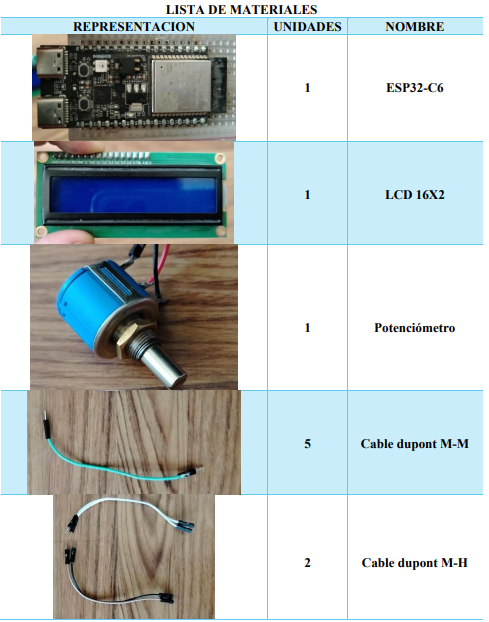
\includegraphics[trim = {0mm 0mm 0mm 0mm},clip,scale=0.5]{12/Img/listaDeMateriales1.png}
        \caption{Lista de materiales}
        \label{fig:listaDeMateriales1.png}
    \end{figure}
    
    \begin{figure}[H]
        \centering
        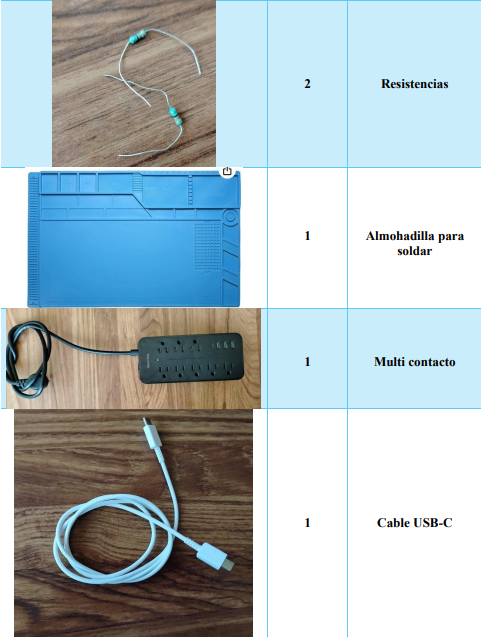
\includegraphics[trim = {0mm 0mm 0mm 0mm},clip,scale=0.5]{12/Img/listaDeMateriales2.png}
        \caption{Lista de materiales}
        \label{fig:listaDeMateriales2.png}
    \end{figure}
    
    \begin{figure}[H]
        \centering
        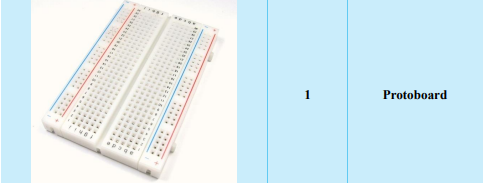
\includegraphics[trim = {0mm 0mm 0mm 0mm},clip,scale=0.5]{12/Img/listaDeMateriales3.png}
        \caption{Lista de materiales}
        \label{fig:listaDeMateriales3.png}
    \end{figure}
    
    \subsection{Descripción de los materiales}
    
    \begin{itemize}
        \item Protoboard: es una placa rectangular con una matriz de orificios conductores. Está diseñado para permitir la conexión temporal de componentes electrónicos sin la necesidad de soldadura. Los orificios están conectados en filas y columnas, facilitando la prototipación rápida y la creación de circuitos electrónicos experimentales. Los componentes se insertan en los orificios y se conectan entre sí utilizando cables de puente. Esto permite una fácil modificación y depuración de los circuitos.\ref{fig:protoboard}
    
          \begin{figure}[H]
            \centering
            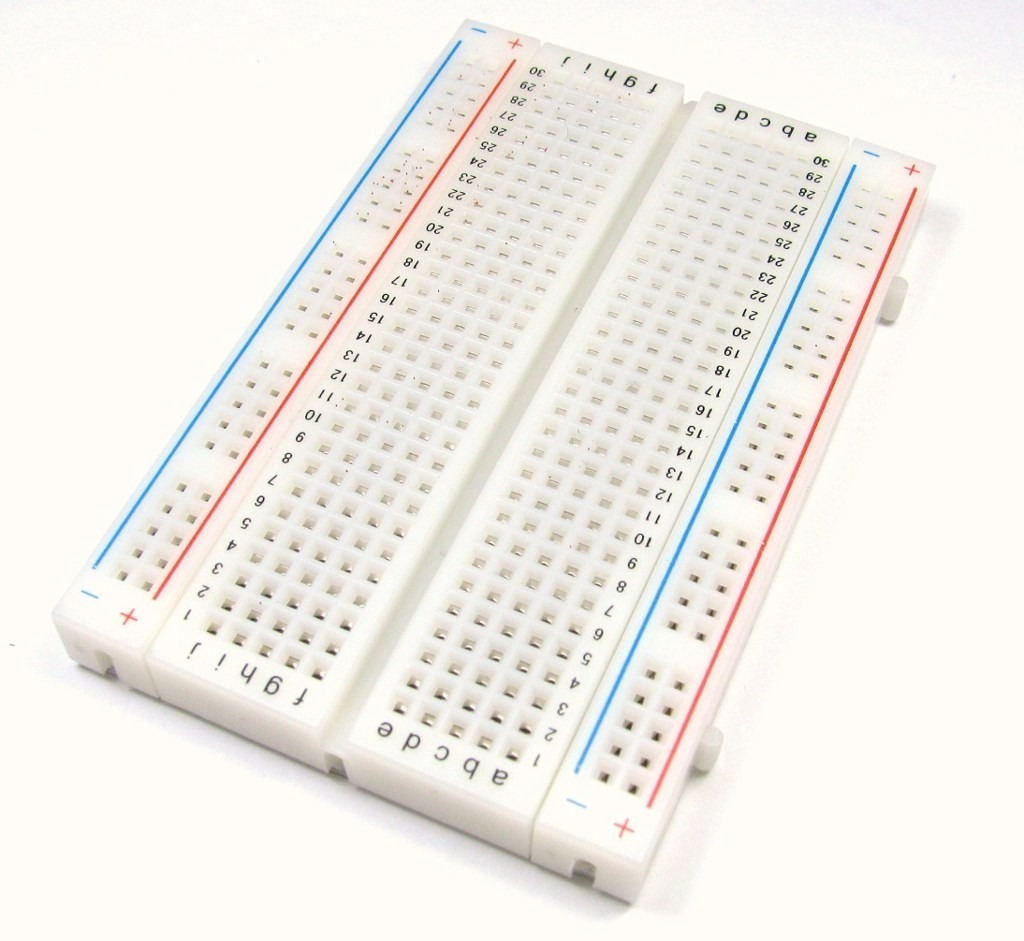
\includegraphics[trim = {0mm 0mm 0mm 0mm},clip,scale=0.2]{12/Img/protoboard.jpg}
            \caption{Imagen representativa del Protoboard}
            \label{fig:protoboard}
        \end{figure}
        
    \end{itemize}
    
    \begin{itemize}
        \item ESP32-C6: Es un microcontrolador de bajo consumo de energía, en el cual sera posicionado en el protoboard, en el cual realizara la tarea de ser receptor y emisor de señal.\ref{fig:ESP32-C6}
    
          \begin{figure}[H]
            \centering
            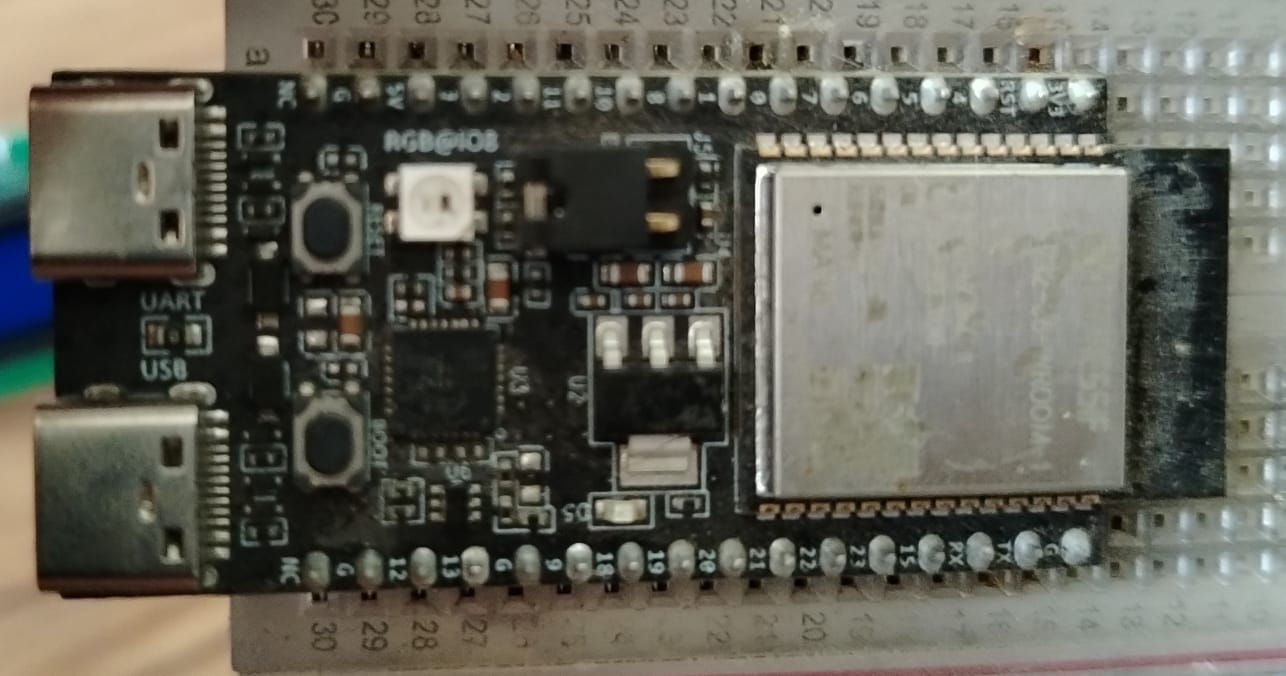
\includegraphics[trim = {0mm 0mm 0mm 0mm},clip,scale=0.2]{12/Img/eSP32-C6.jpg}
            \caption{Imagen representativa del ESP32-C6}
            \label{fig:ESP32-C6}
        \end{figure}
        
    \end{itemize}
    
    \begin{itemize}
        \item Resistencia: Se trata de un componente de plástico con alambre que se utiliza en circuitos eléctricos para controlar o modificar el flujo de corriente eléctrica. Al insertarse en los orificios del protoboard, este elemento proporciona una ruta alternativa para la corriente, lo que puede disminuir su intensidad o direccionarla según sea necesario para el funcionamiento deseado del circuito.\ref{fig:Resistencia}
    
          \begin{figure}[H]
            \centering
            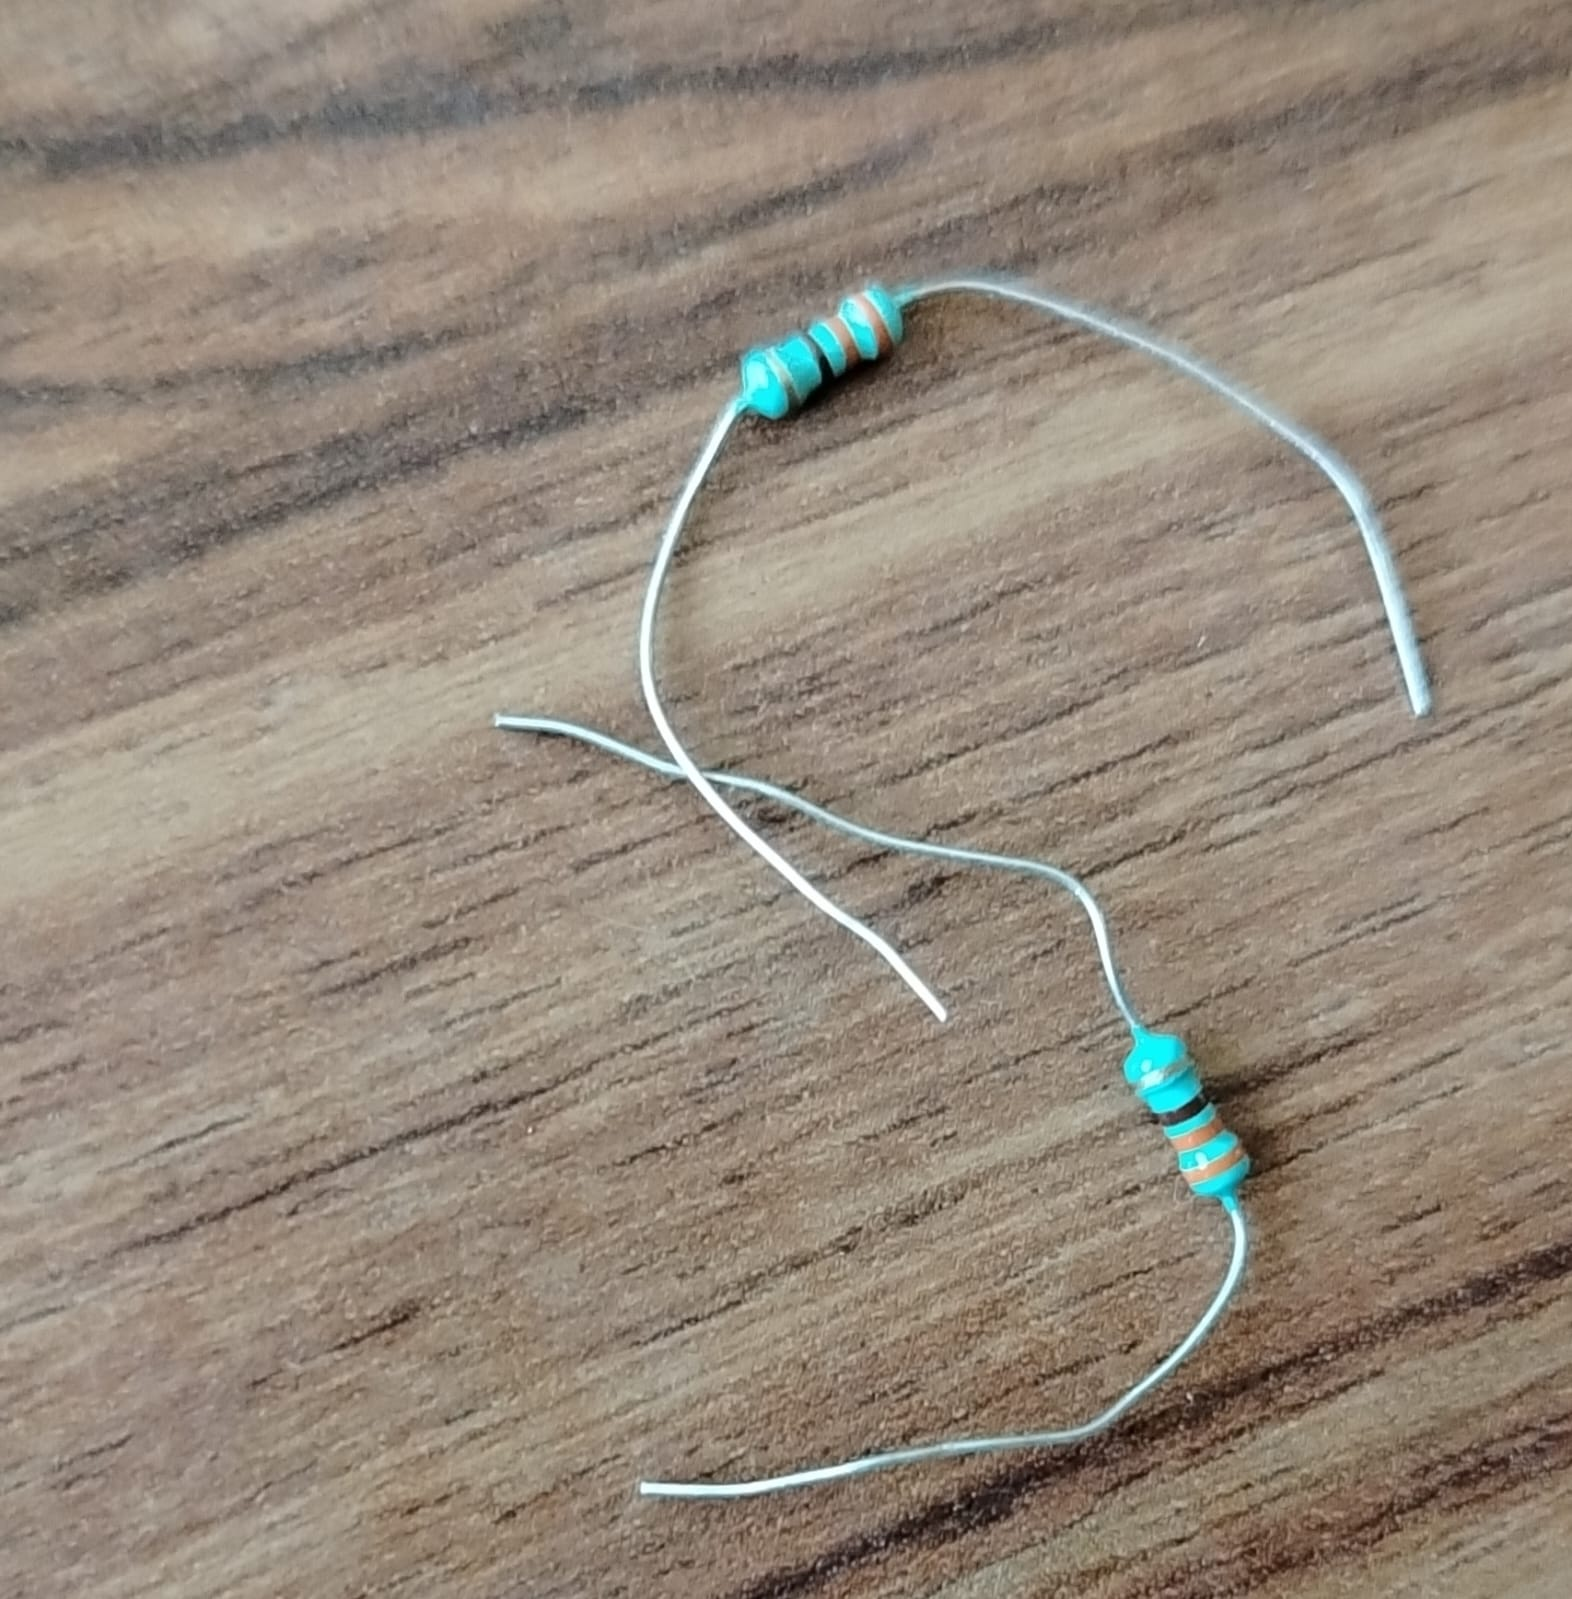
\includegraphics[trim = {0mm 0mm 0mm 0mm},clip,scale=0.1]{12/Img/resistencia.jpg}
            \caption{Imagen representativa de la Resistencia}
            \label{fig:Resistencia}
        \end{figure}
    \end{itemize}
    
    \begin{itemize}
        \item Cable dupont M-M:  tipo de cable específicamente diseñado para la interconexión de componentes en circuitos eléctricos. Este cable cuenta con una varilla metálica en cada extremo, lo que facilita su conexión directa entre dos puntos del protoboard sin necesidad de soldadura. Este diseño permite una conexión rápida y segura entre los elementos del circuito, lo que resulta especialmente útil en la fase de prototipo y pruebas. \ref{fig:CableDupontMM}
    
          \begin{figure}[H]
            \centering
            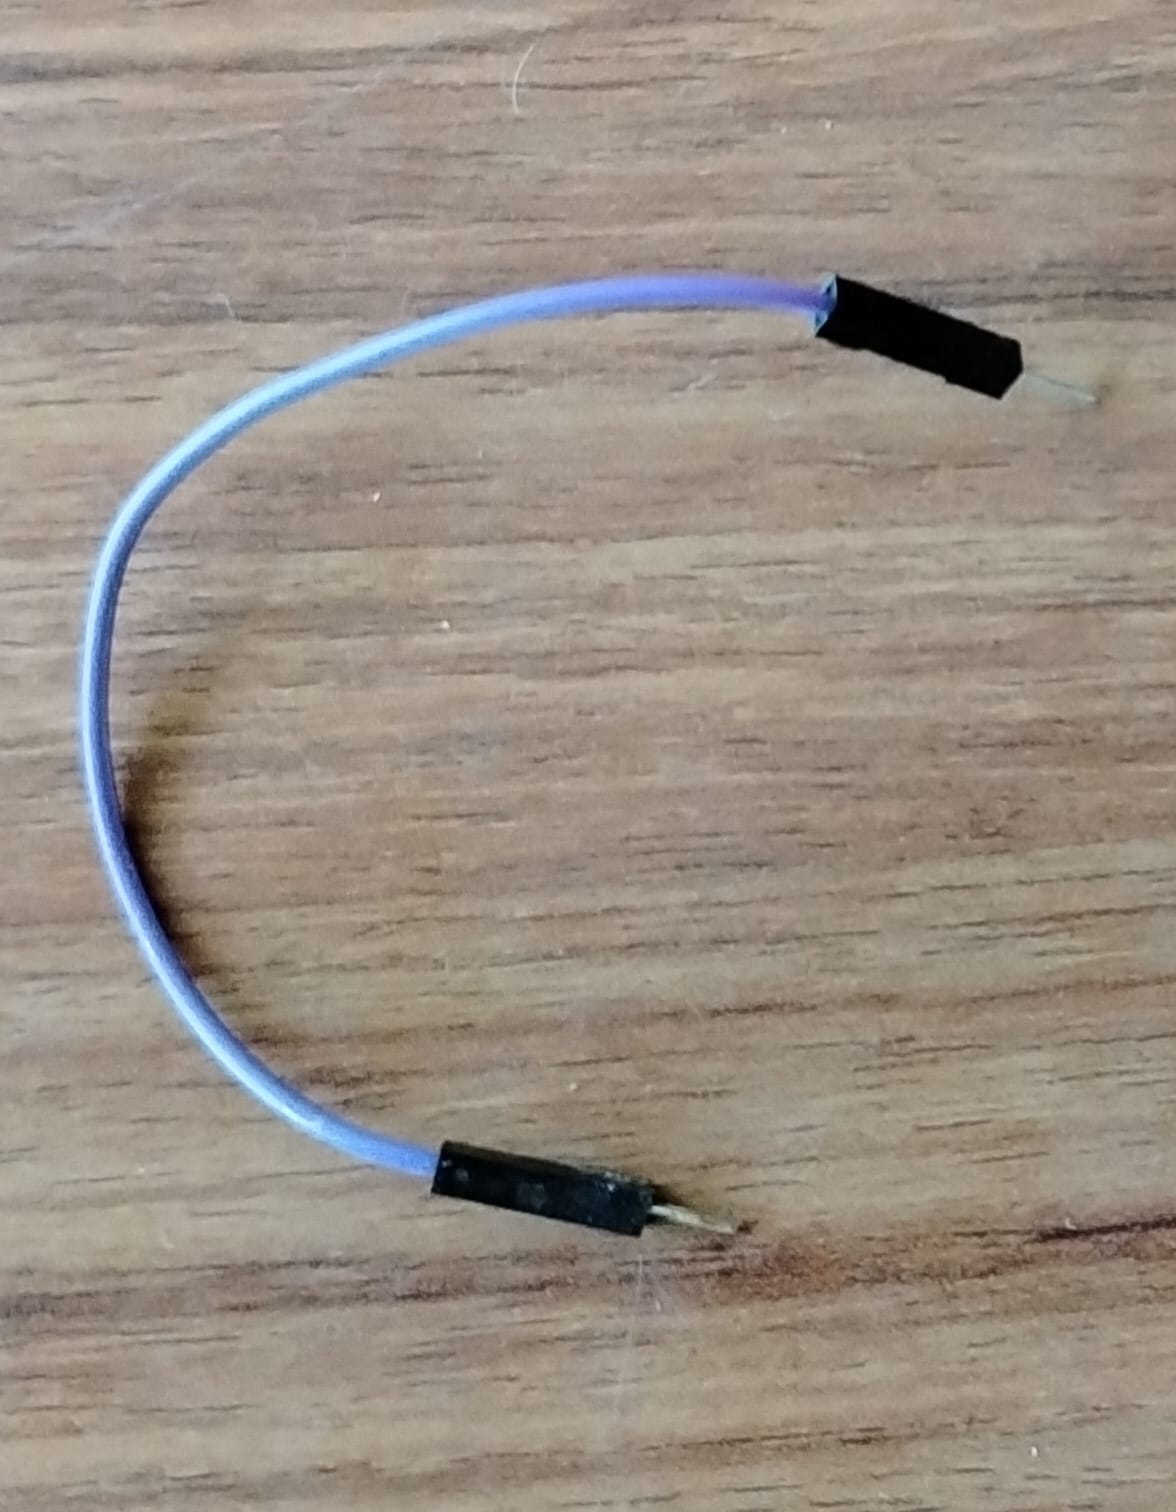
\includegraphics[trim = {0mm 0mm 0mm 0mm},clip,scale=0.1]{12/Img/cableDupontMM.jpg}
            \caption{Imagen representativa de Cable Dupont M-M}
            \label{fig:CableDupontMM}
        \end{figure}
    \end{itemize}
    
    \begin{itemize}
        \item Cable dupont M-H: Este tipo de cable se emplea en la construcción de circuitos eléctricos y se caracteriza por tener una varilla metálica únicamente en uno de sus extremos. Esta disposición lo convierte en una opción comúnmente utilizada como extensión para conectar otros cables a una mayor distancia en un protoboard. Al insertar el extremo sin la varilla en el orificio del protoboard, el extremo con la varilla se conecta a otro cable o componente, permitiendo así la expansión y flexibilidad en la disposición de los elementos dentro del circuito.  \ref{fig:CableDupontMH}
    
          \begin{figure}[H]
            \centering
            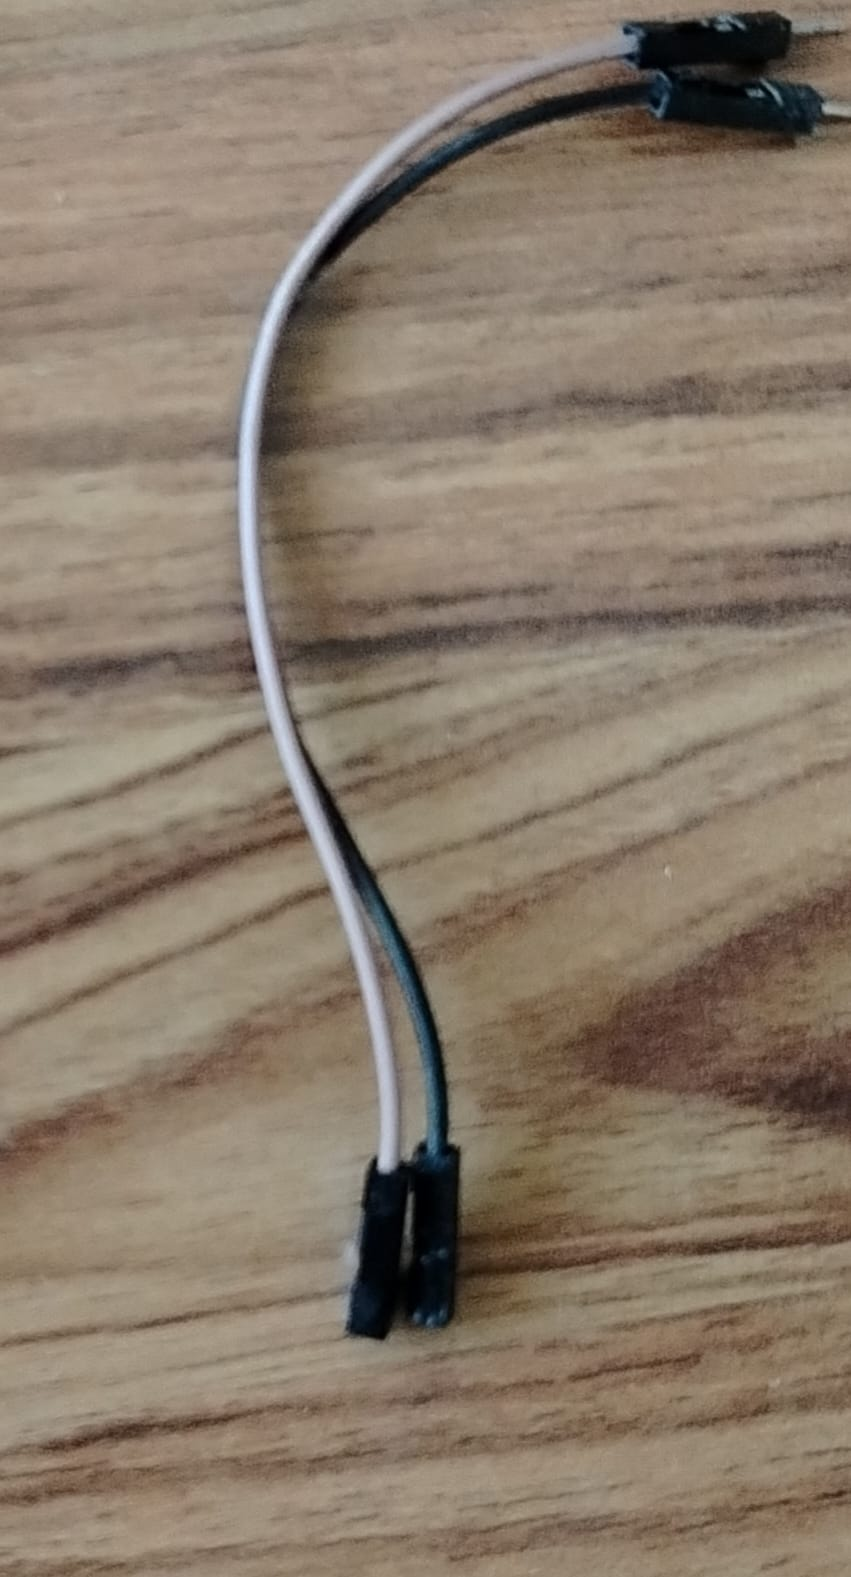
\includegraphics[trim = {0mm 0mm 0mm 0mm},clip,scale=0.1]{12/Img/cableDupontMH.jpg}
            \caption{Imagen representativa de Cable Dupont M-H}
            \label{fig:CableDupontMH}
        \end{figure}
    \end{itemize}
    
    \begin{itemize}
        \item Potenciómetro: Similar a una resistencia, el potenciómetro tiene la capacidad de ajustar su valor de resistencia eléctrica. Sin embargo, a diferencia de una resistencia estándar con un valor fijo, el potenciómetro es variable y puede ser ajustado manualmente. Esto permite modificar la resistencia en el circuito de acuerdo a las necesidades específicas de la aplicación. Al girar el eje del potenciómetro, se altera la posición de un contacto deslizante sobre una resistencia resistiva, lo que cambia la longitud efectiva del conductor eléctrico. Esta característica lo convierte en una herramienta útil para controlar variables como el brillo de una lámpara, el volumen de un altavoz, o la velocidad de un motor, entre otros ejemplos. El potenciómetro se utiliza comúnmente para mantener una corriente controlada dentro del circuito, permitiendo ajustes precisos en tiempo real según las demandas específicas del sistema.  \ref{fig:Potenciometro}
    
          \begin{figure}[H]
            \centering
            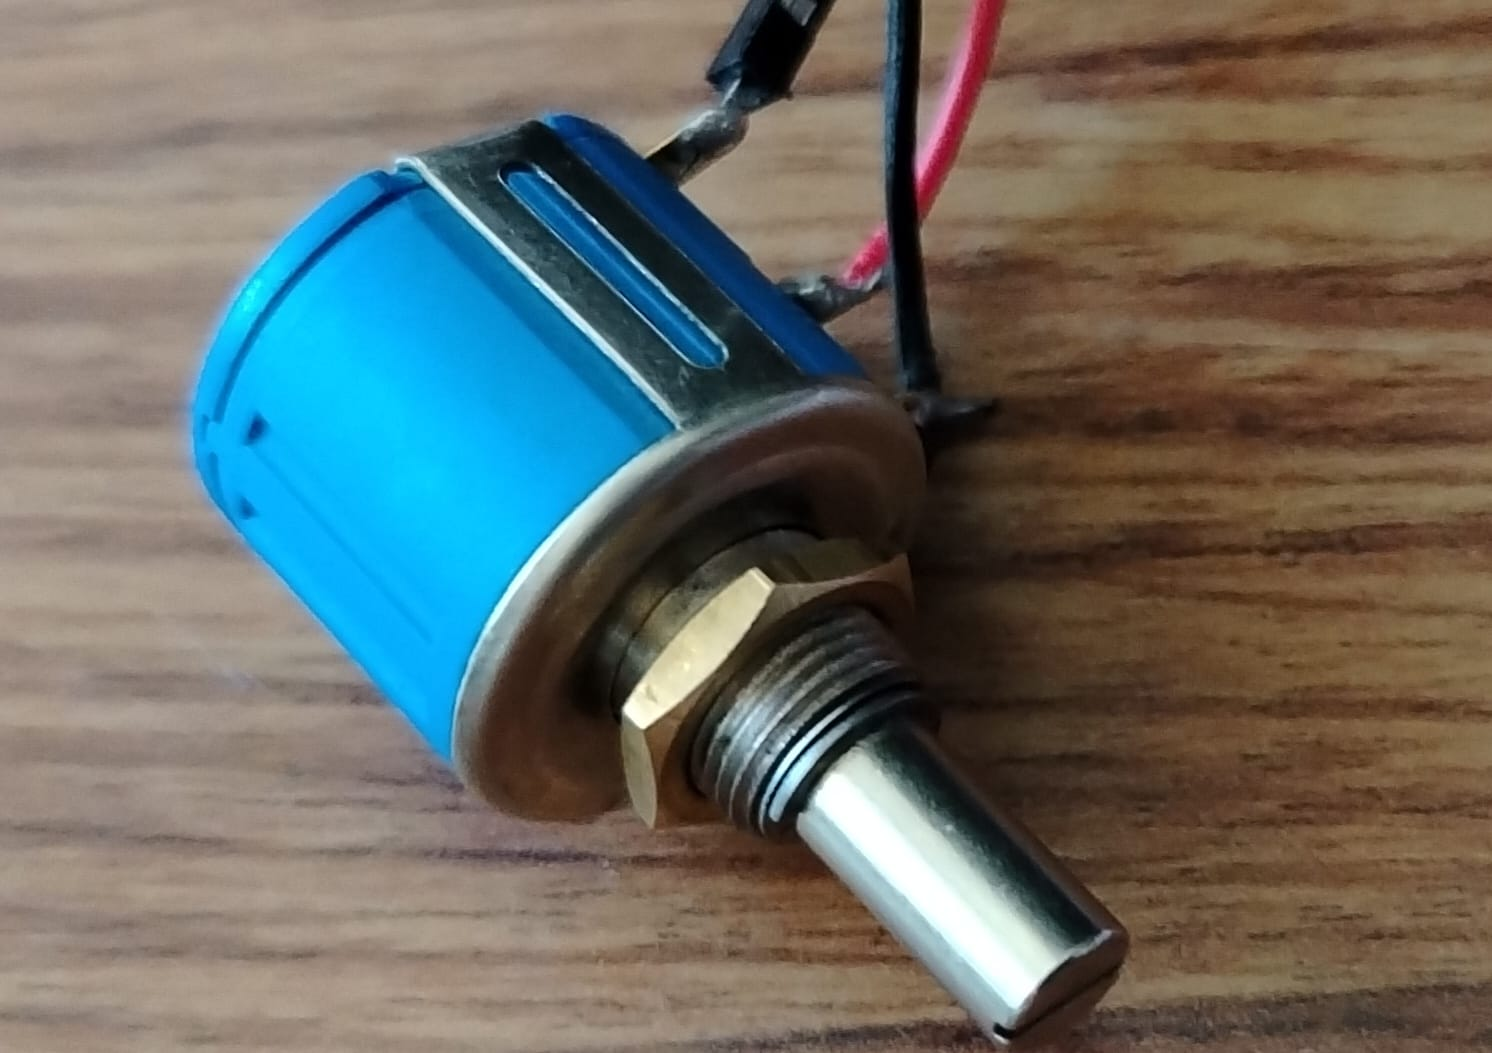
\includegraphics[trim = {0mm 0mm 0mm 0mm},clip,scale=0.1]{12/Img/potenciometro.jpg}
            \caption{Imagen representativa de Potenciometro}
            \label{fig:Potenciometro}
        \end{figure}
    \end{itemize}
    
    \begin{itemize}
        \item LCD: Este componente electrónico se utiliza principalmente en circuitos eléctricos para visualizar información de manera clara y legible.  \ref{fig:LCD}
    
          \begin{figure}[H]
            \centering
            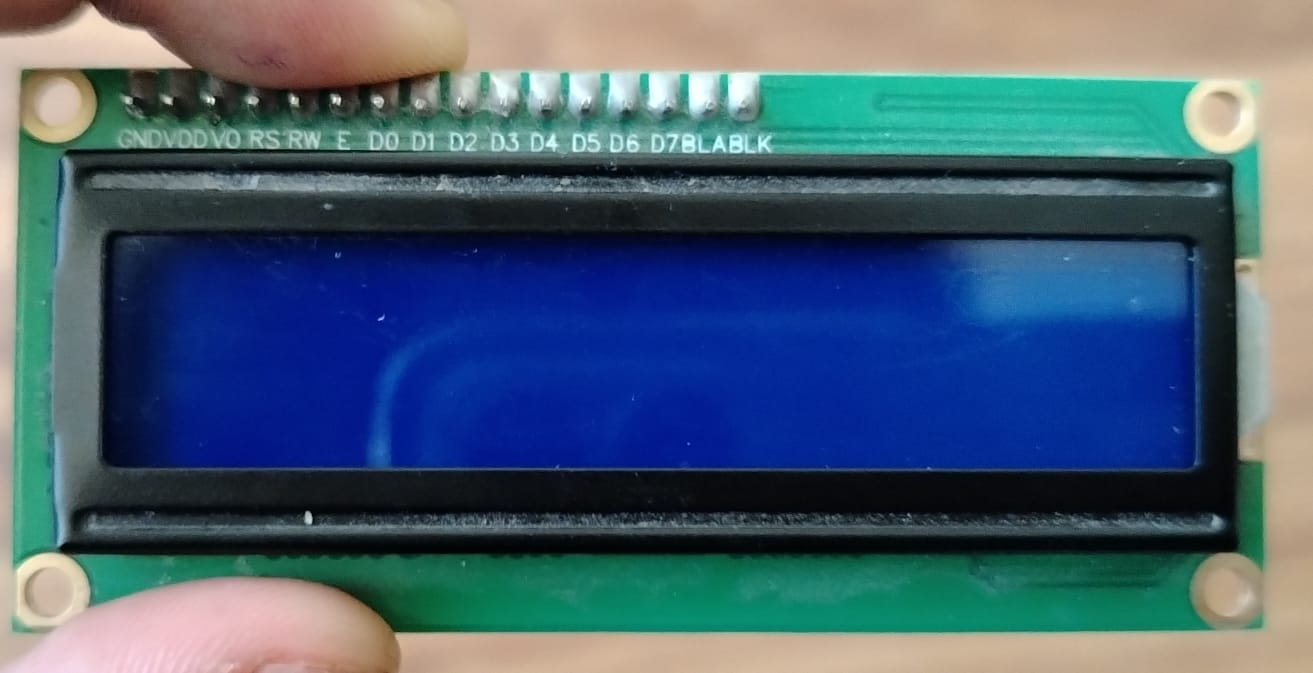
\includegraphics[trim = {0mm 0mm 0mm 0mm},clip,scale=0.15]{12/Img/lcd.jpg}
            \caption{Imagen representativa del LCD}
            \label{fig:LCD}
        \end{figure}
    \end{itemize}
    
    \begin{itemize}
        \item Extensión multi contacto: Herramienta de transmisión de fuente eléctrica que alimentara al circuito. \ref{fig:extensión}
    
          \begin{figure}[H]
            \centering
            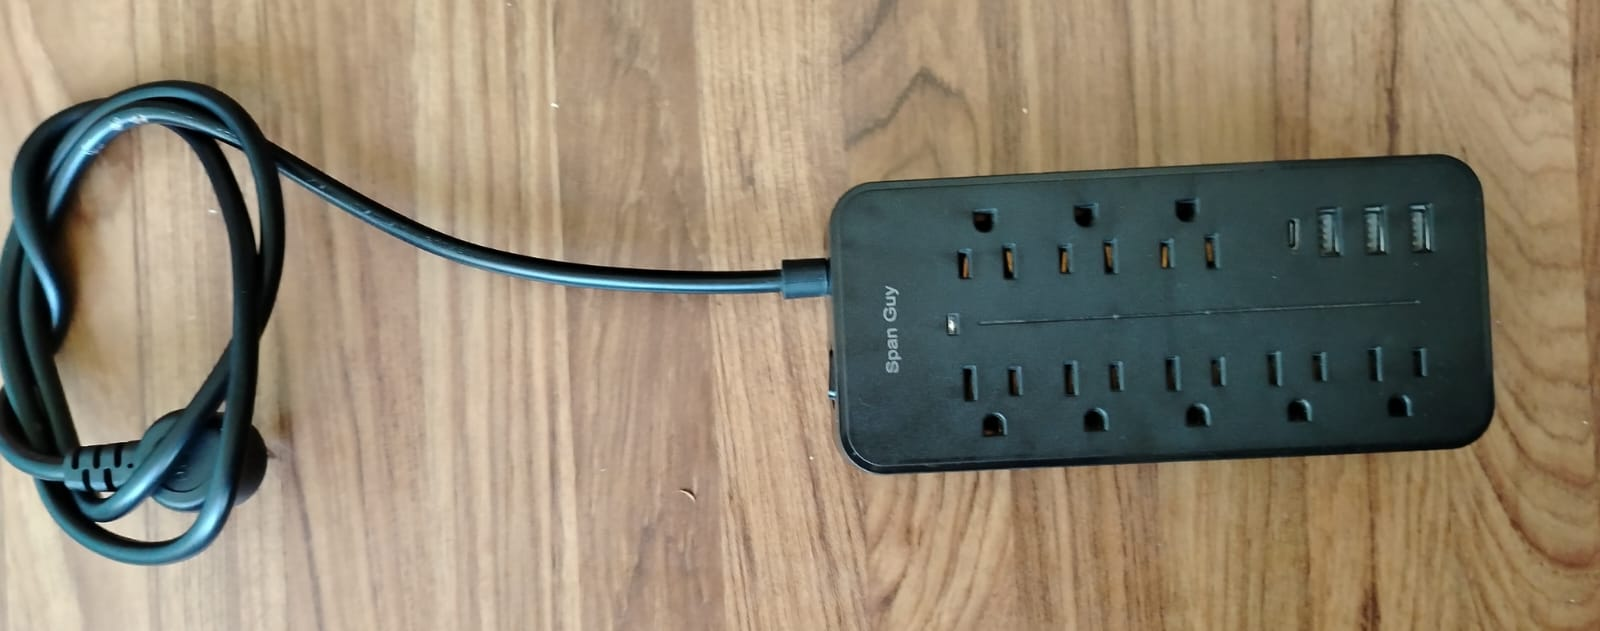
\includegraphics[trim = {0mm 0mm 0mm 0mm},clip,scale=0.15]{12/Img/extensionMultiContacto.jpg}
            \caption{Imagen representativa de la Extensión}
            \label{fig:extensión}
        \end{figure}
    \end{itemize}
    
    \begin{itemize}
        \item Cable USBC: Cable para brindarle una fuente de energía al circuito.  \ref{fig:USBC}
    
          \begin{figure}[H]
            \centering
            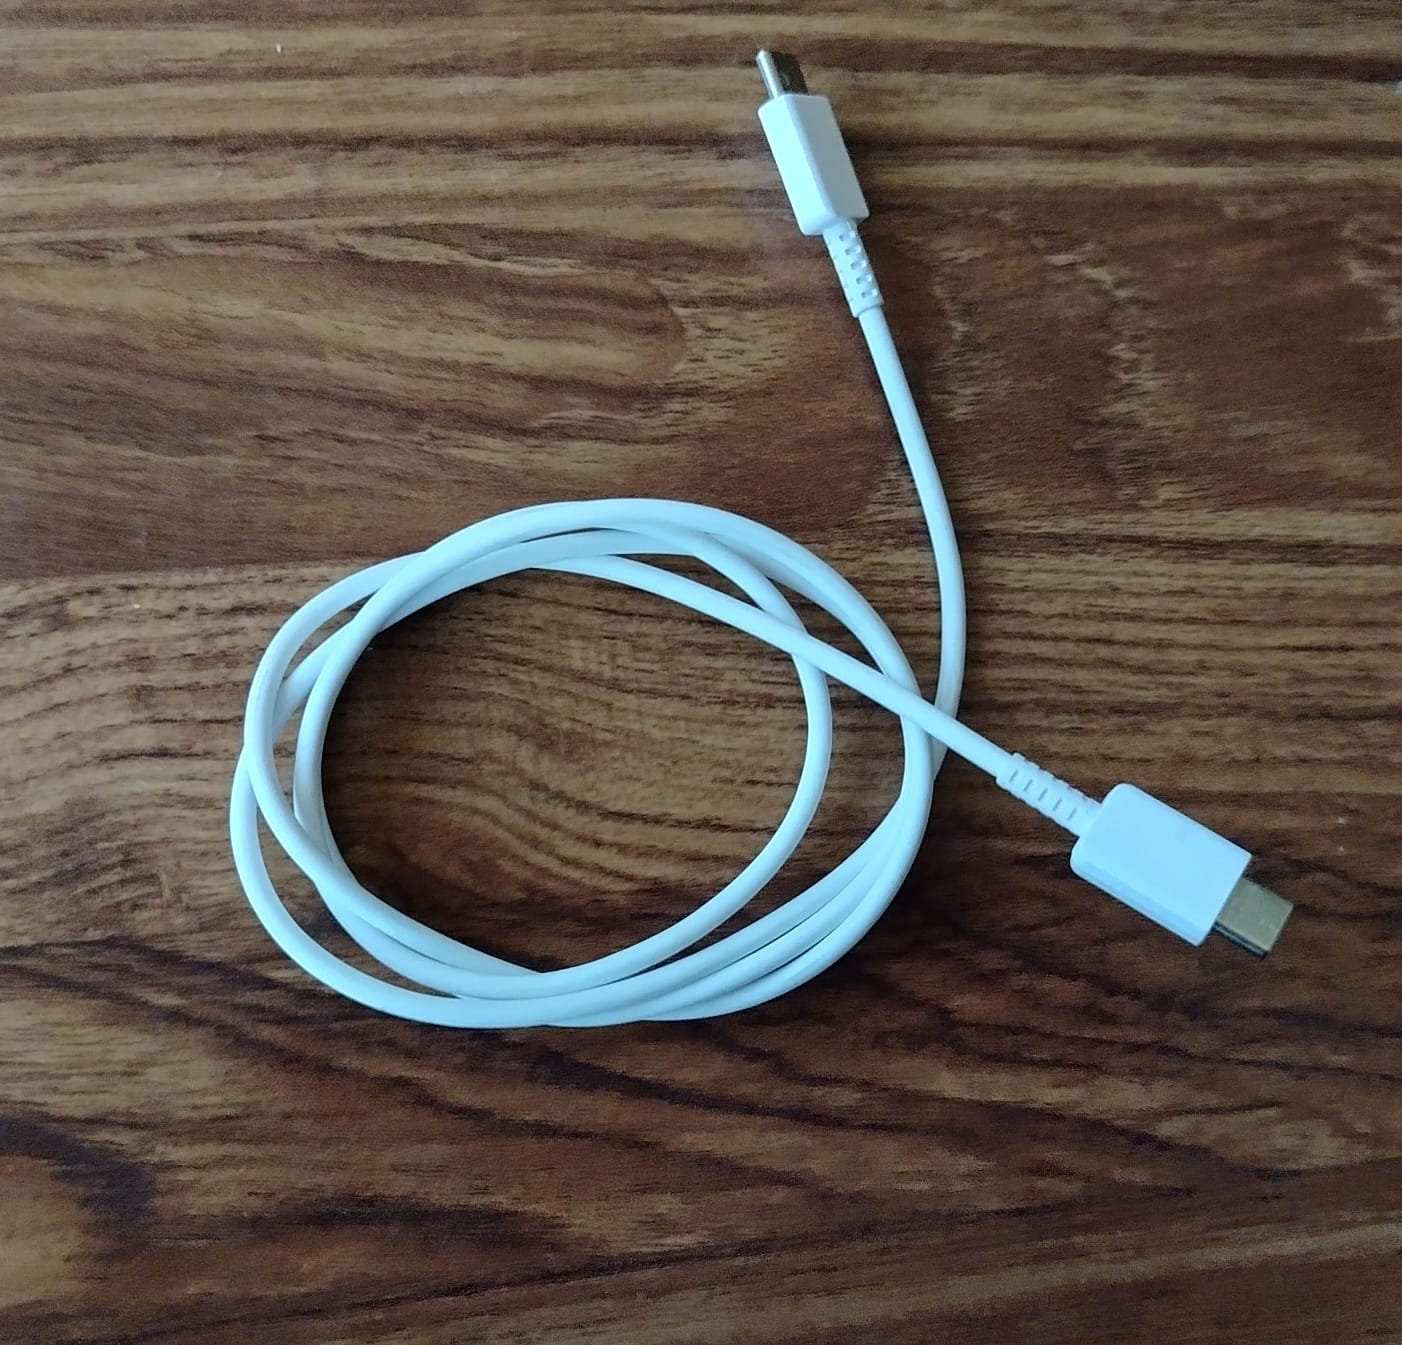
\includegraphics[trim = {0mm 0mm 0mm 0mm},clip,scale=0.1]{12/Img/cableUsbc.jpg}
            \caption{Imagen representativa de la Extensión}
            \label{fig:USBC}
        \end{figure}
    \end{itemize}
    
    \begin{itemize}
        \item Modulo I2C: Este módulo actúa como una interfaz que simplifica la integración y el manejo de las pantallas LCD en los circuitos electrónicos.\ref{fig:modulo}
    
          \begin{figure}[H]
            \centering
            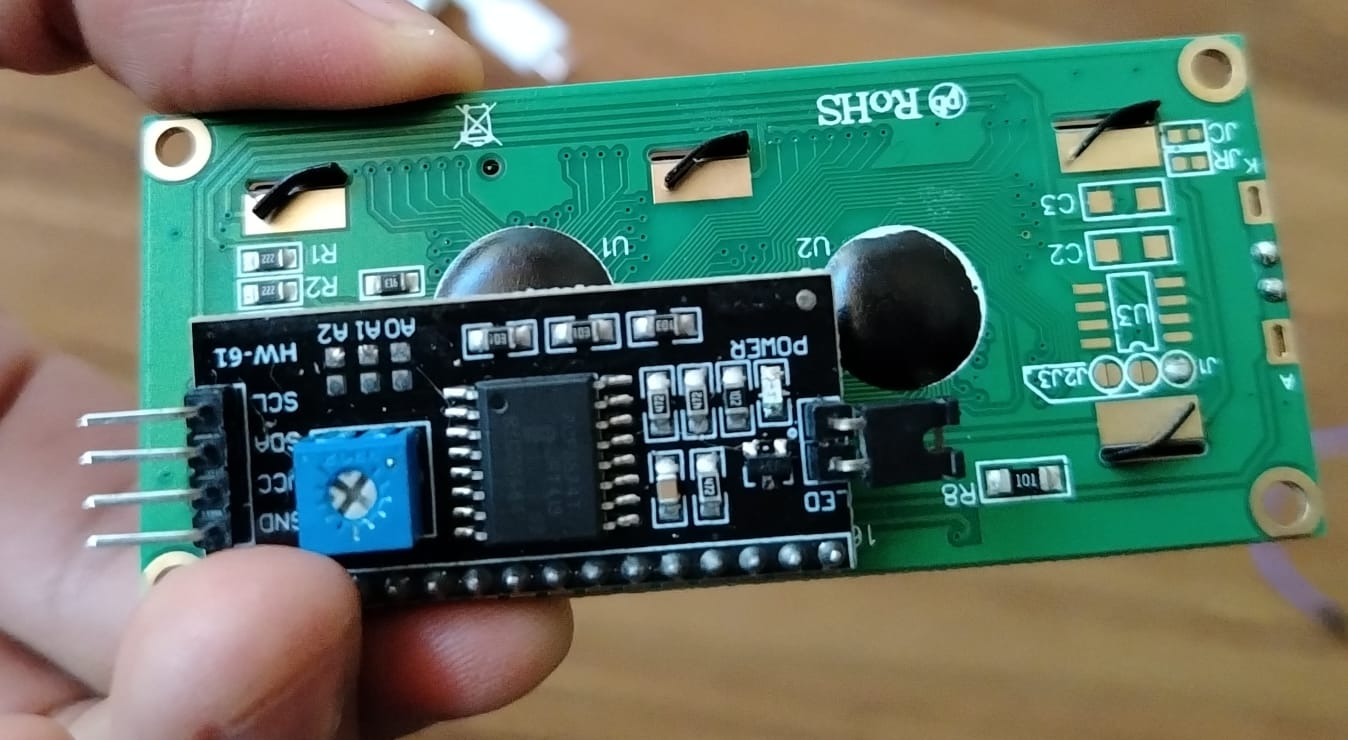
\includegraphics[trim = {0mm 0mm 0mm 0mm},clip,scale=0.15]{12/Img/moduloI2C.jpg}
            \caption{Imagen representativa de la Extensión}
            \label{fig:modulo}
        \end{figure}
    \end{itemize}
    
    \subsection{Procedimiento de ensamble}
    \begin{itemize}
        \item Paso 1. Conectar el multi contacto a una fuente de energía.
        \item Paso 2. Conectar el ESP32-C6 al protoboard.
        \item Paso 3. Conectar los pines de alimentación VCC y GND.
        \item Paso 4. Conectar el potenciómetro a la protoboard, y mediante los extremos del potenciómetro conectar el VCC y GND,junto con la central del pin analógico del ESP32-C6.
        \item Paso 5.Conectar la LCD al protoboard junto con las resistencias y condensores, Luego los pines de datos de series (I2C) y los pines de control al ESP32.
        \item Paso 6. Conectar el cable USB-C al multi contacto que le brindara la energía al ESP32.
        \item Paso 7. Al realizar la acción con el potenciómetro verificar que este funcione y haga la lectura indicada. 
    \end{itemize}
    Mediante este proceso debemos adquirir los resultados necesarios hasta llegar al esperado, dado que en el ensamble se pueden cometer errores se debe tener una correcta documentación para percibir áreas de mejora en el proceso.
    
    %Cada estrategia metodológica se establece acorde a cada objetivo, y por tanto deberá ser desglosada precisada y ordenada claramente. En consecuencia cada objetivo que se presentó en forma de verbo en infinitivo deberá determinar una estrategia en forma de adverbio. Ej. Desarrollar…Desarrollo. Son las actividades ordenadas que tienen como finalidad la prueba de la hipótesis. 
    
    %\begin{itemize}
        %\item Se debe establecer que se habrá de hacer, como, conque, y donde para obtener la información que permita probar la hipótesis.  
        %\item Se debe desglosar de acuerdo a los objetivos específicos. 
        %\item Se debe establecer una estrategia metodológica por cada objetivo específico. De manera simplista se podría decir que se cambia el verbo en infinitivo por su respectivo adverbio.
        %\item En cada objetivo se debe describir que método, que materiales y que equipo se usará para conseguirlo.
        %\item Se deben tener referencias Figura \ref{fig:lcd-16x2}.
    %\end{itemize}
    % 
    % 
    %\begin{figure}[H]
        %\centering
        %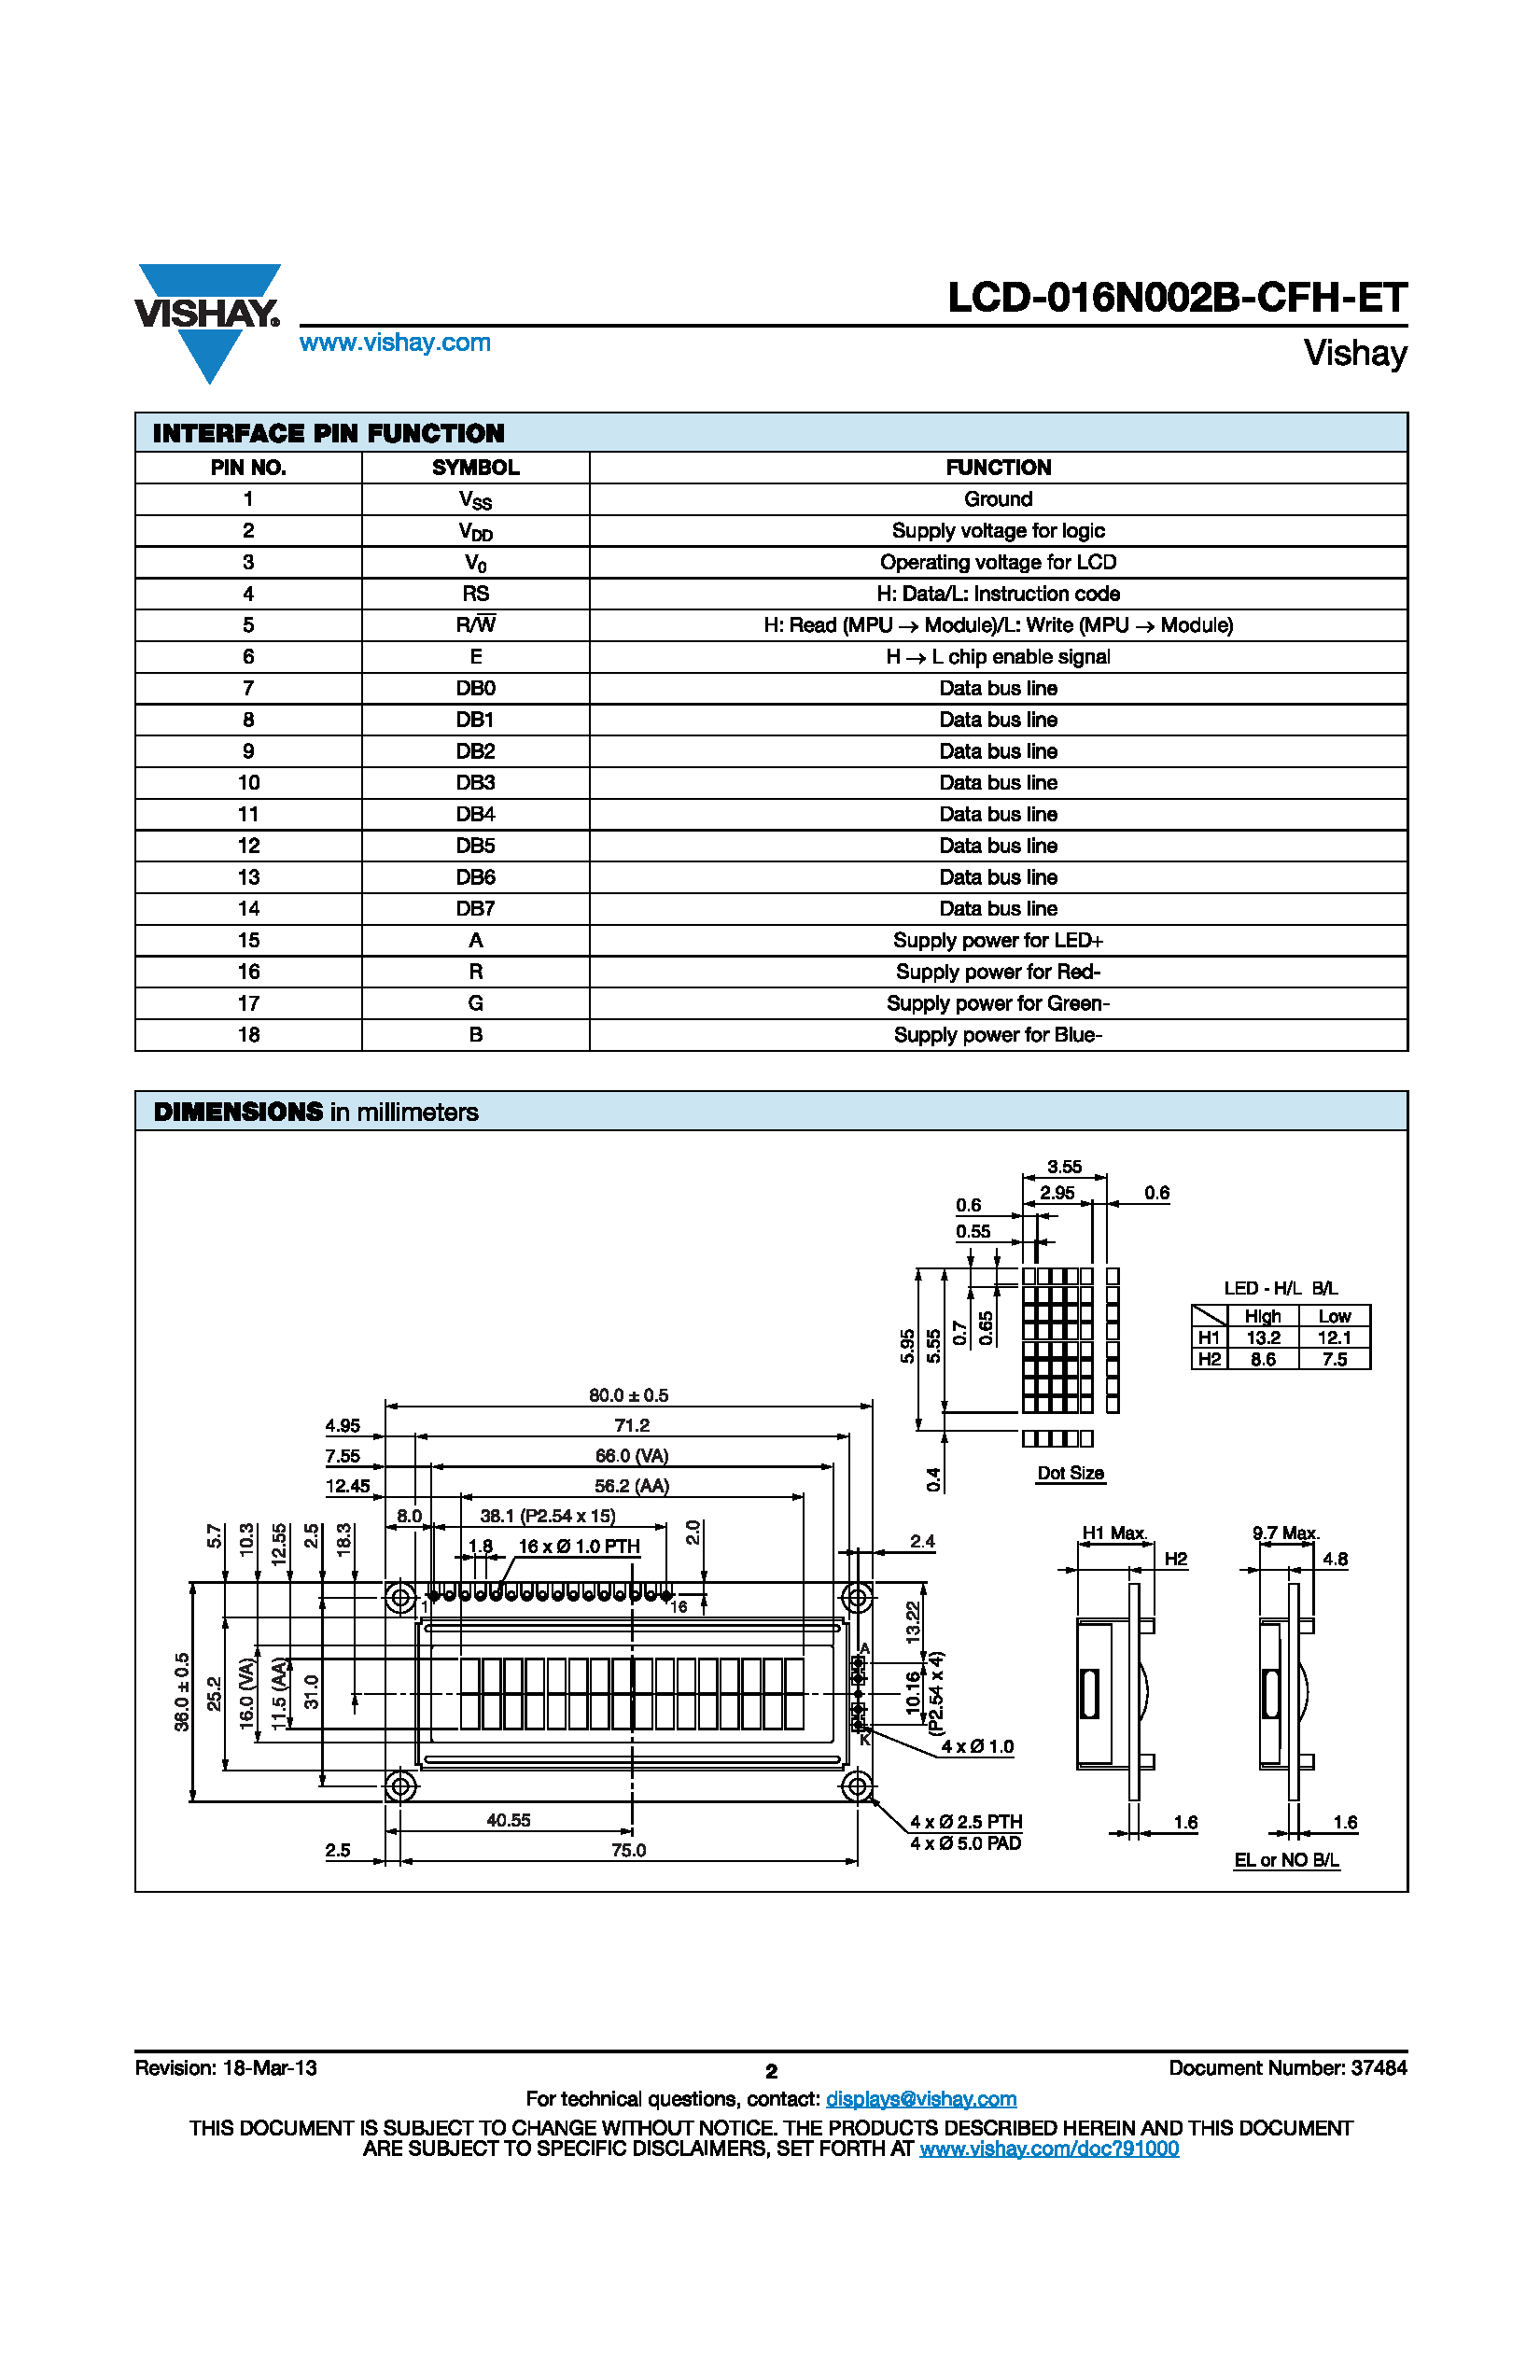
\includegraphics[trim = {30mm 65mm 90mm 250mm},clip,scale=0.5]{6/Img/lcd-16x2.pdf}
        %\caption{Esquema LCD de 16x2}
        %\label{fig:lcd-16x2}
    %\end{figure}
    % 
    % 
    %\begin{figure}[H]
        %\centering
        %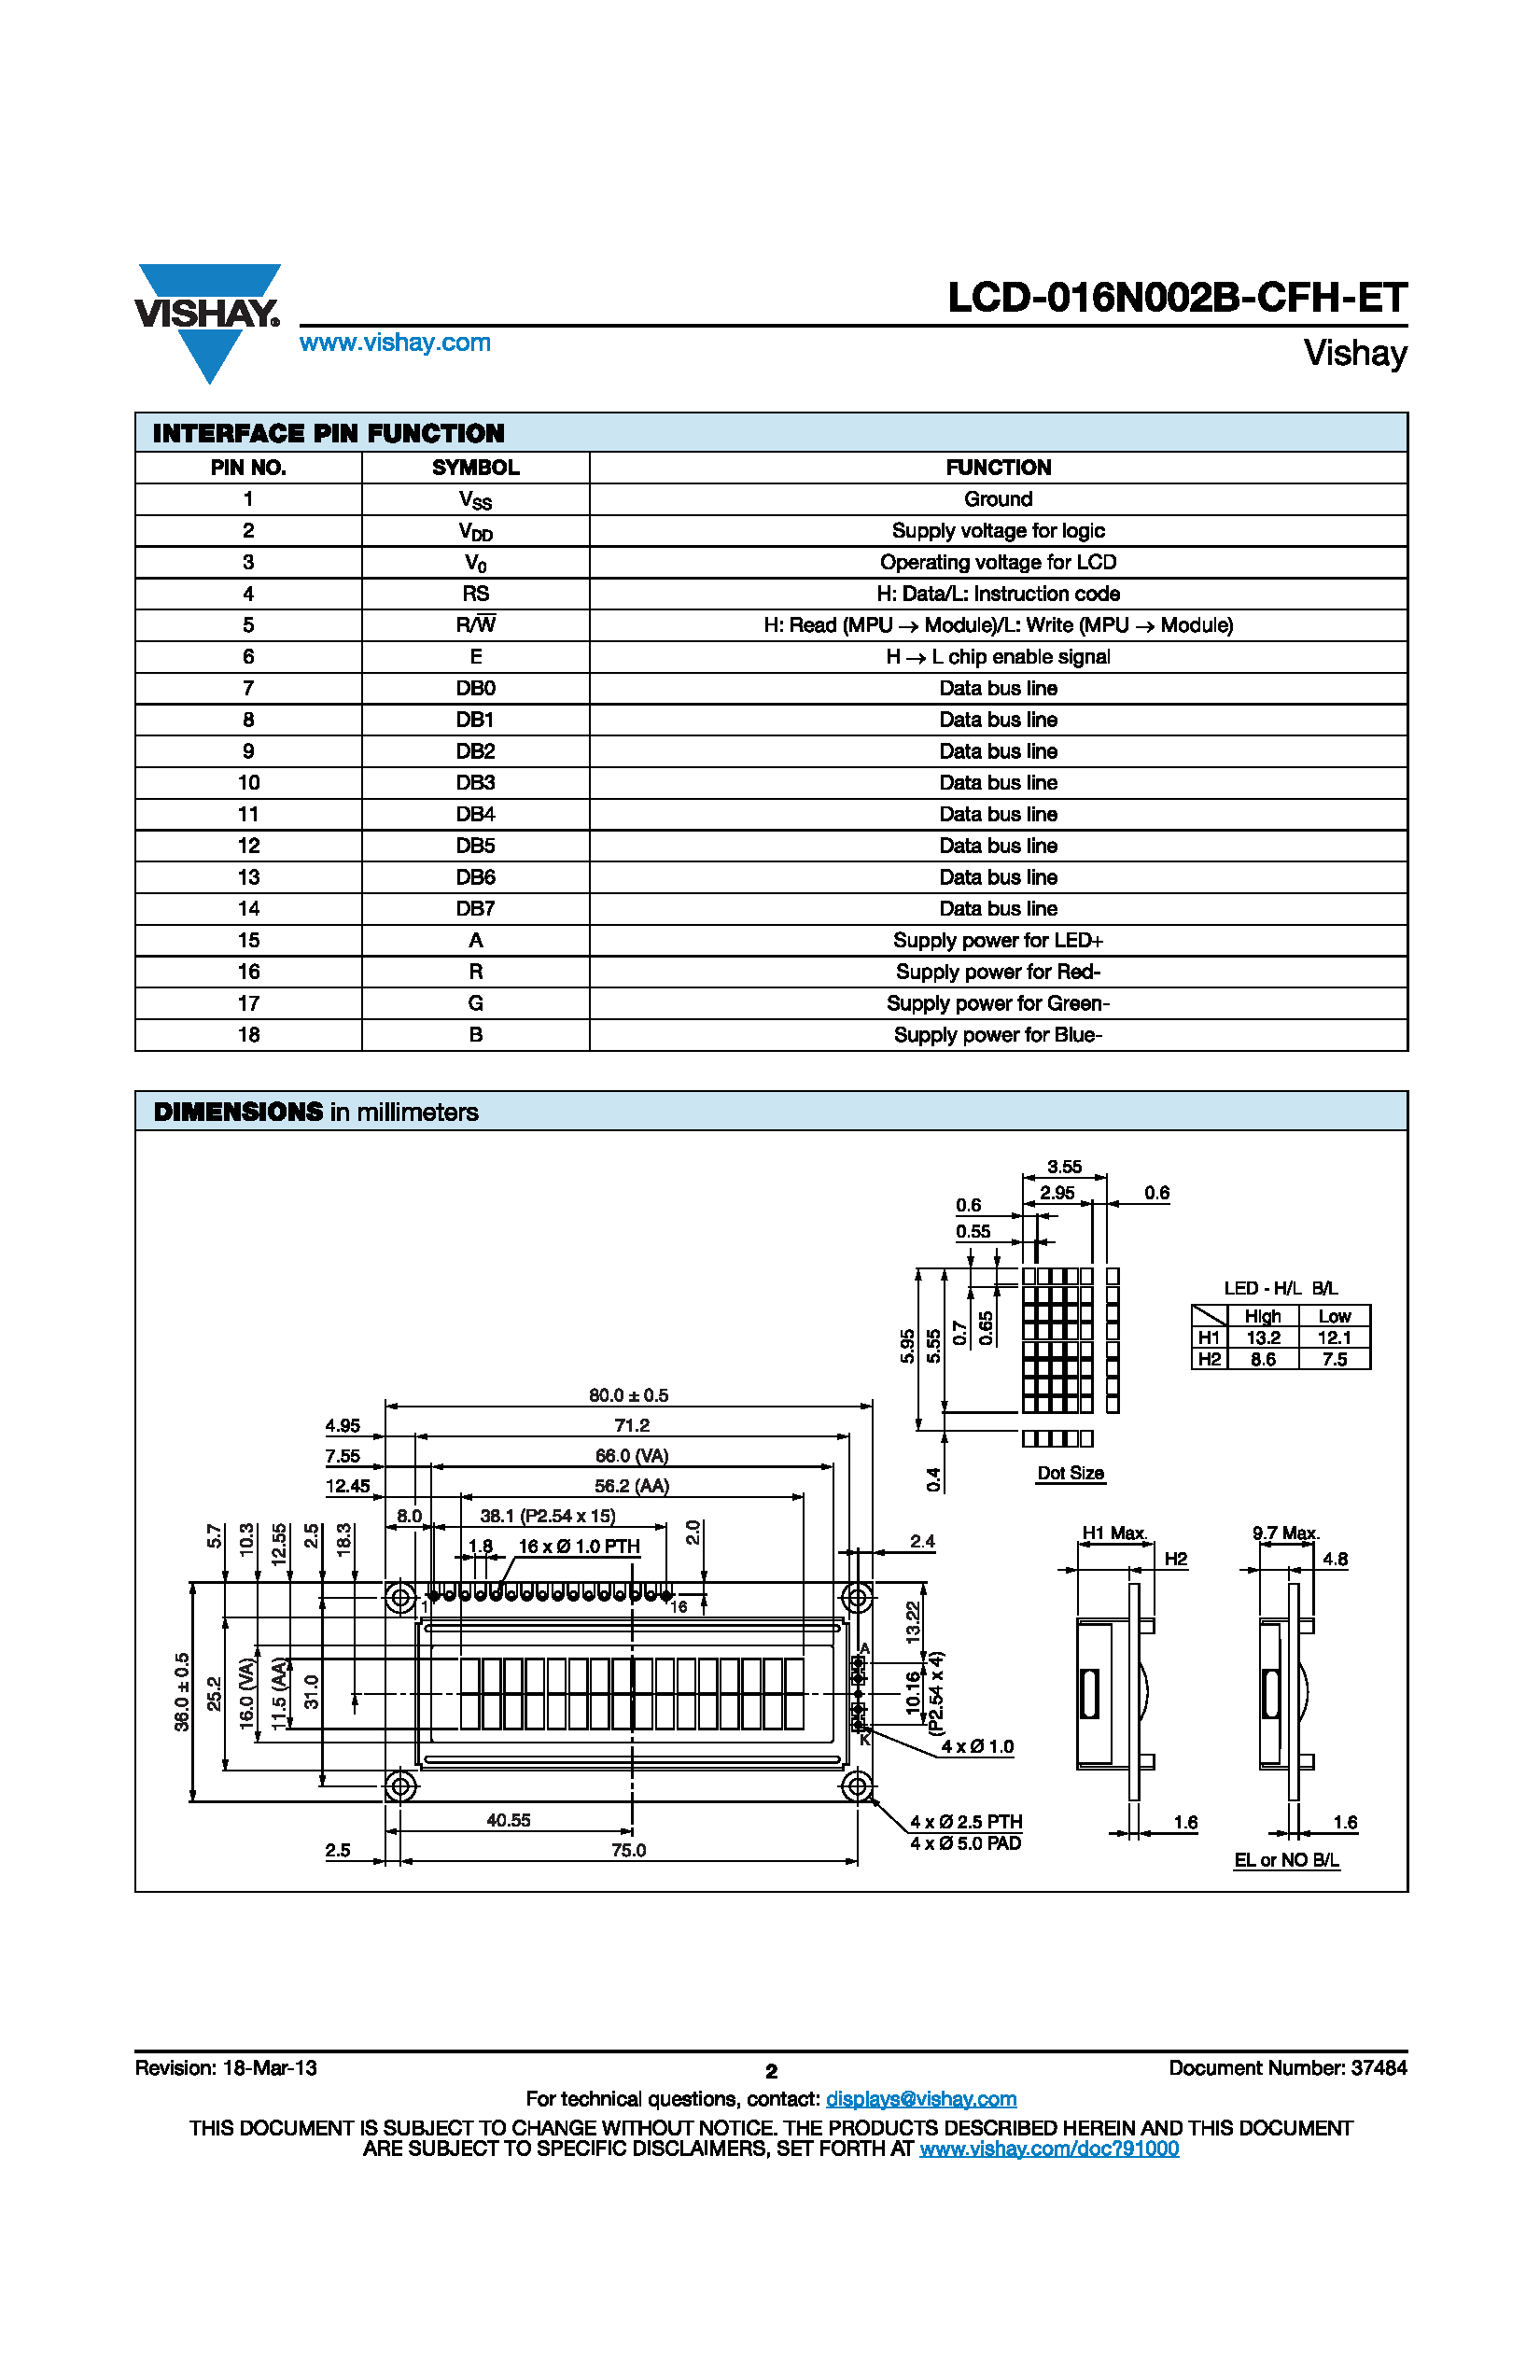
\includegraphics[trim = {30mm 250mm 90mm 20mm},clip,scale=0.5]{6/Img/lcd-16x2.pdf}
        %\caption{Esquema LCD de 16x2}
        %\label{fig:lcd-16x2}
    %\end{figure}
    % 
    % 
    %\subsection{Prepara tu documento}
    
    %Antes de que comiences a utilizar esta plantilla, es recomendable que prepare la información que contendrá en un archivo aparte. 
    %Ten preparadas tus gráficas, así como también las tablas aparte, para que sea más fácil integrarlo. 
    %Se recomienda fuertemente el uso de \textbf{formato Enhanced Metafile (.emf) para imágenes y gráficas} de resolución óptima. 
    %Finalmente, completa y organiza el contenido antes de darle el formato de esta plantilla. 
    
    \subsection{Acrónimos y Abreviaciones}
    
    Los acrónimos y abreviaciones deberán ser definidos únicamente la primera vez que aparecen en el texto, esto para que el lector entienda lo que significan.
    
    \subsection{Ecuaciones}
    
    %Las ecuaciones son una excepción a las especificaciones prescritas de esta plantilla. 
    %Deberá determinar si su ecuación debe escribirse o no utilizando la fuente Adobe Devangari. 
    %Para crear ecuaciones multinivel, puede ser necesario tratar la ecuación como un gráfico e insertarla en el texto después de aplicar el estilo de la platilla.
    %Las ecuaciones serán enumeradas de manera consecutiva, y el número de ecuación, entre paréntesis, se colocan al ras de la derecha, utilizando una tabulación derecha. 
    Después de esta preparación, el operador iniciará el proceso de ensamblaje. El analista estará listo con una tabla para registrar los tiempos de cada paso y un cronómetro para medir la duración de cada actividad.
    
    El proceso continuará hasta que el operador complete el ensamblaje del circuito, marcando así la conclusión de un ciclo de producción. Se llevarán a cabo varios ciclos para recopilar datos significativos.
    
    Posteriormente, se compararán los valores obtenidos en cada ciclo. Utilizando una fórmula específica, se calculará el valor esperado. Esta fórmula considerará los tiempos registrados en cada paso del proceso y proporcionará una estimación del tiempo total esperado para el ensamblaje del circuito. Este valor esperado servirá como referencia para evaluar y mejorar la eficiencia del proceso de ensamblaje.
    \begin{equation}
        \label{eq1}
         (X1+X2+...+Xn)/n 
    \end{equation}
    
    Una vez recopilados los datos de cada ciclo, se procederá a calcular la media de los tiempos obtenidos. Esta media representará el tiempo esperado para llevar a cabo el ensamblaje del circuito utilizando la metodología de tiempos continuos.
    
    Esta cifra promedio servirá como punto de referencia crucial para evaluar la eficiencia del proceso actual. Siempre y cuando el tiempo real de ensamblaje se aproxime al tiempo esperado, se puede concluir que la metodología de tiempos continuos está funcionando adecuadamente. Por otro lado, si existen discrepancias significativas entre el tiempo real y el esperado, esto puede indicar áreas donde se pueden realizar mejoras en el proceso de ensamblaje.
    %Es importante asegurarse de que los símbolos de la ecuación sean definidos antes o inmediatamente después de la ecuación. Utilice “(1)”, en vez de “Eq. 1” al enumerar las ecuaciones, excepto al principio de una oración: “La ecuación (\ref{eq1}) es…”
    
    \section{Resultados y discusión}
    espués de que el operario haya leído detenidamente el manual de fabricación, analizado su contenido y memorizado las instrucciones, procederá a ensamblar el circuito de forma manual. Durante este proceso, el operario se basará exclusivamente en las instrucciones previamente proporcionadas, sin recibir ningún tipo de ayuda externa. Mientras tanto, un analista observará atentamente y grabará un vídeo continuo para evaluar si el operario lleva a cabo cada paso del ensamblaje de manera correcta.
    
    Una vez completado el ensamblaje, para verificar su adecuada realización, el operario realizará una modificación en el rango del potenciómetro. Esto implicará ajustar el potenciómetro y modificar su resistencia para observar cómo esto afecta la lectura en la pantalla. El analista tomará evidencia tanto de la funcionalidad apropiada de la pantalla LCD al encenderse y recibir la señal como del efecto de la variación de la resistencia del potenciómetro en la lectura, tal como se ilustra en la imagen adjunta.\ref{fig:evidencia5}
    
    \begin{figure}[H]
            \centering
            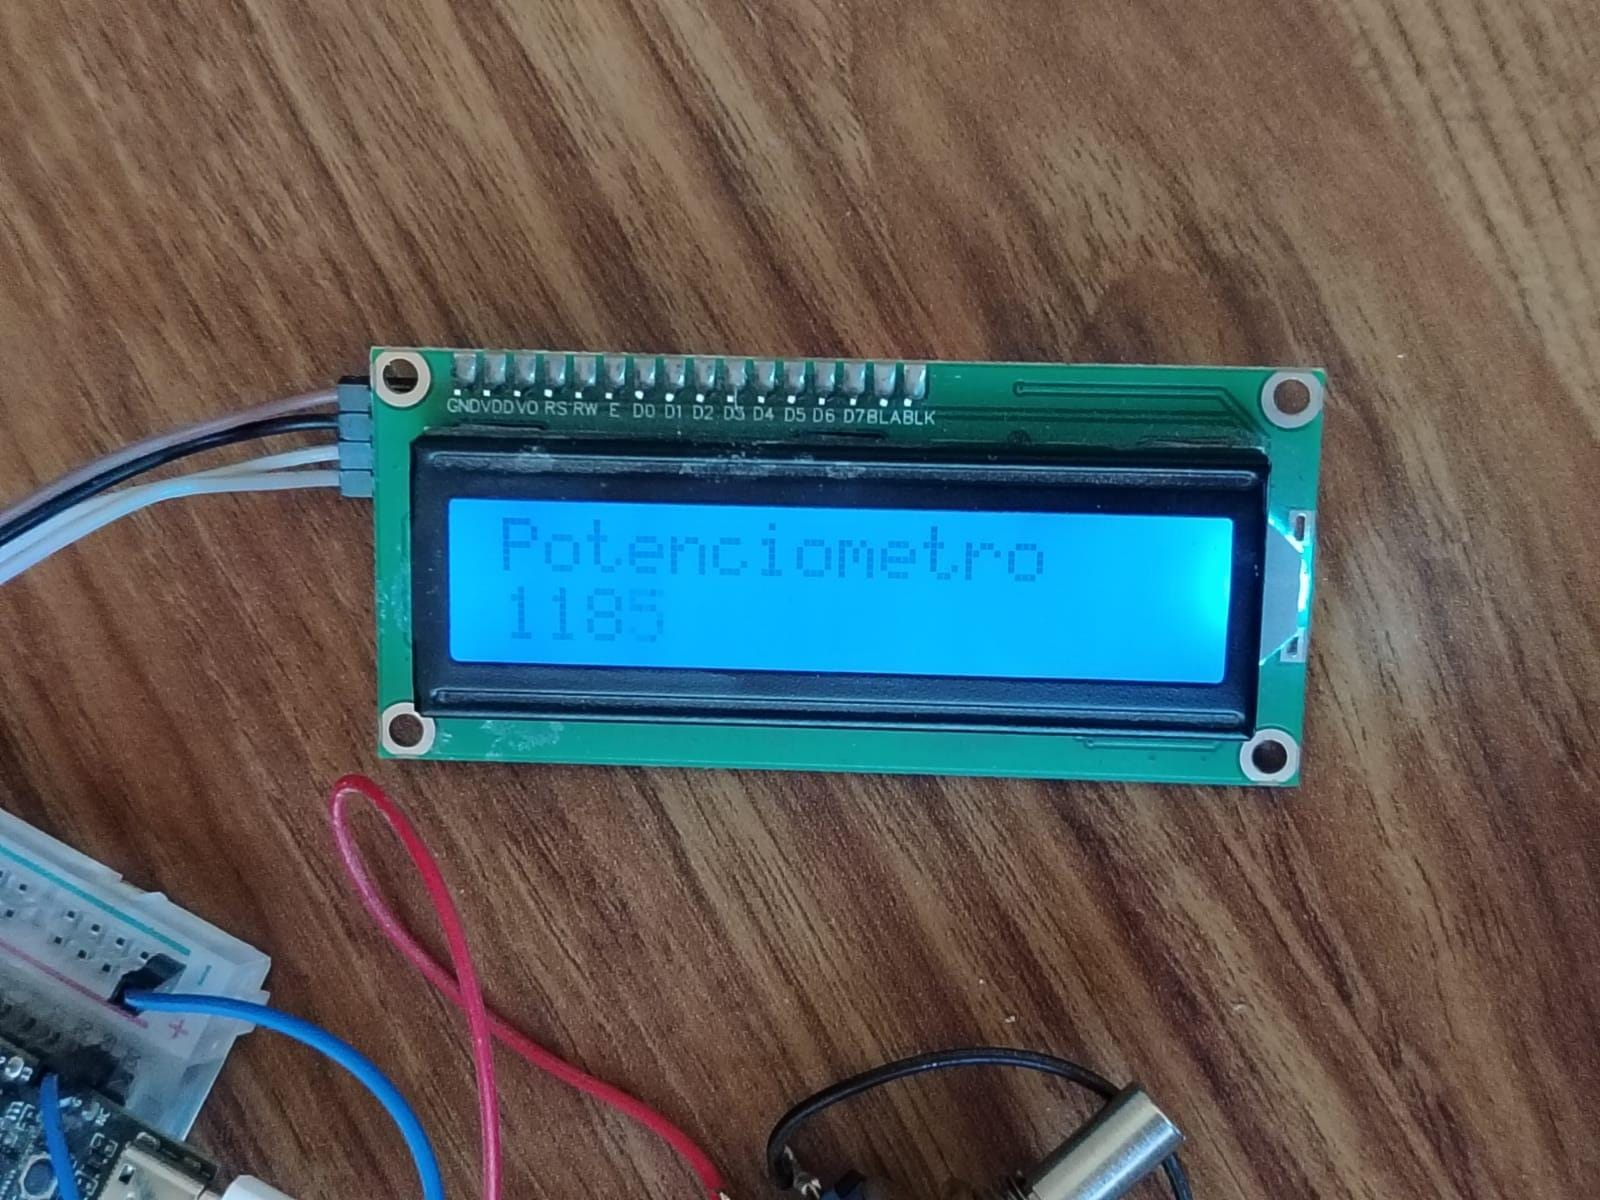
\includegraphics[trim = {0mm 0mm 0mm 0mm},clip,scale=0.15]{12/Img/evidencia5.jpg}
            \caption{Lectura en pantalla LCD}
            \label{fig:evidencia5}
    \end{figure}
    
    De forma complementaria se adjuntaran algunas imágenes(\ref{fig:evidencia1})(\ref{fig:evidencia2})(\ref{fig:evidencia3})(\ref{fig:evidencia4}) del proceso de ensamble, para que sirvan de evidencia que el ensamble fue realizado de forma adecuada. También como una medida correctiva en caso de que algún elemento del proceso fue realizado de manera equivocada y así brindar retroalimentación y corrección en el manual del ensamble. 
    
    \begin{figure}[H]
            \centering
            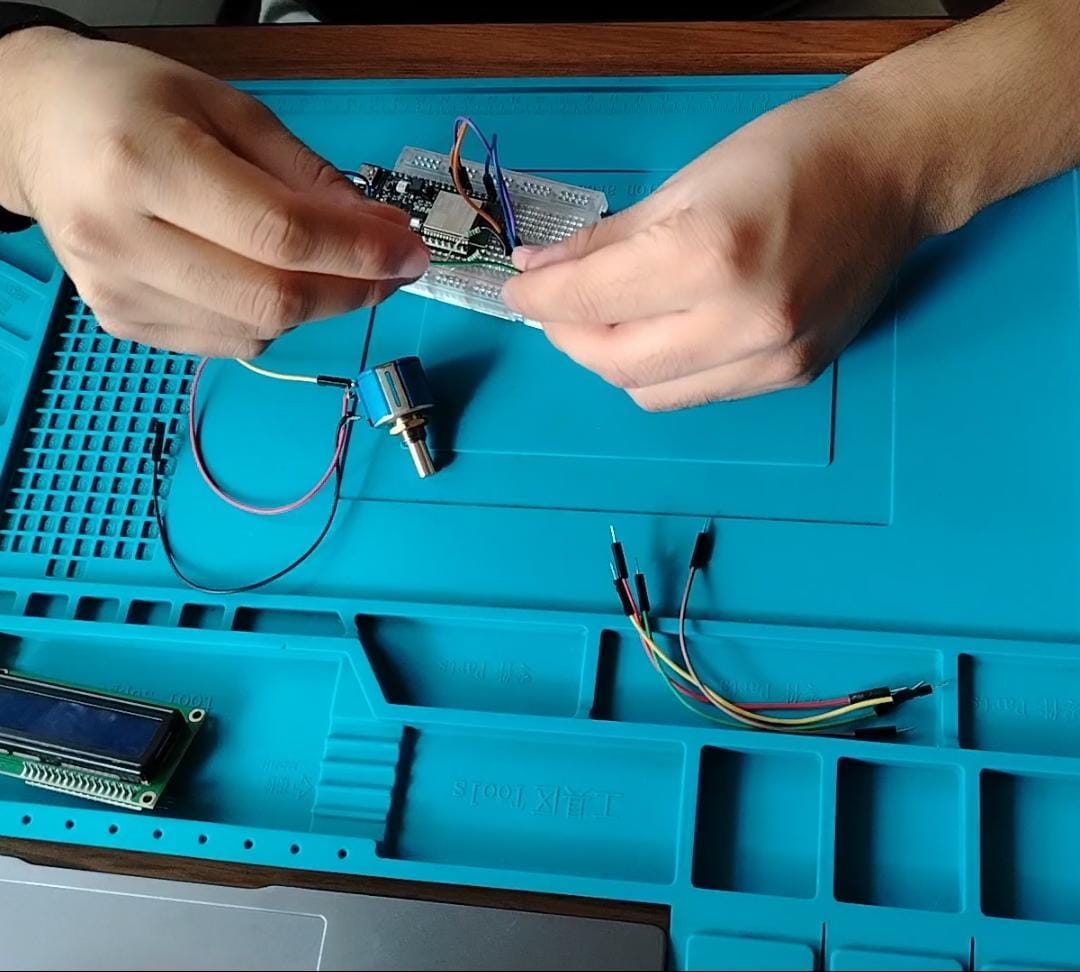
\includegraphics[trim = {0mm 0mm 0mm 0mm},clip,scale=0.2]{12/Img/evidencia1.jpg}
            \caption{Evidencia del proceso de ensamble}
            \label{fig:evidencia1}
    \end{figure}
    
    \begin{figure}[H]
            \centering
            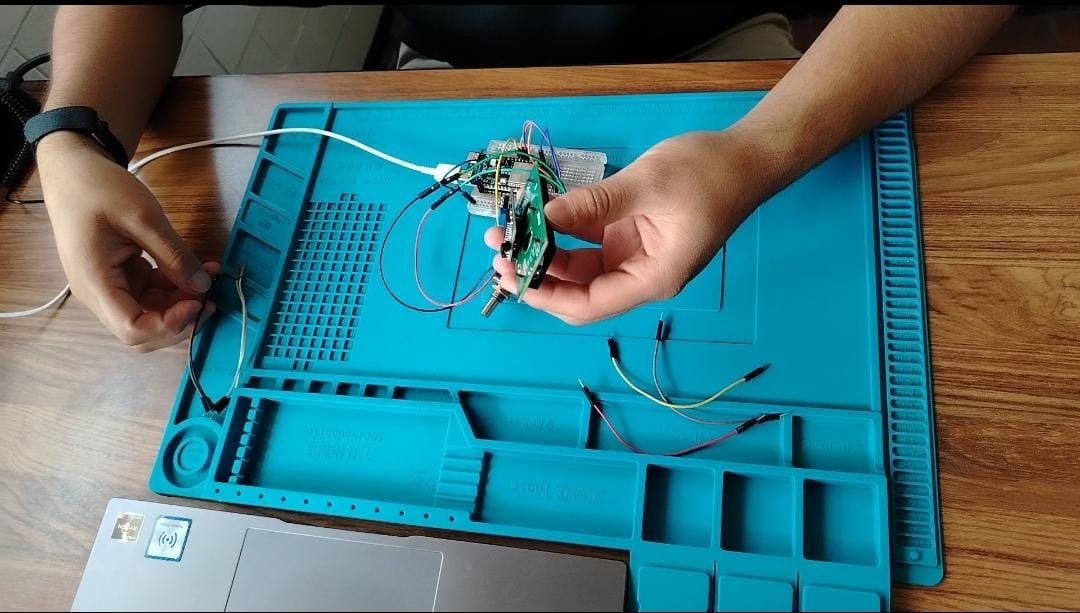
\includegraphics[trim = {0mm 0mm 0mm 0mm},clip,scale=0.2]{12/Img/evidencia2.jpg}
            \caption{Evidencia del proceso de ensamble}
            \label{fig:evidencia2}
    \end{figure}
    
    \begin{figure}[H]
            \centering
            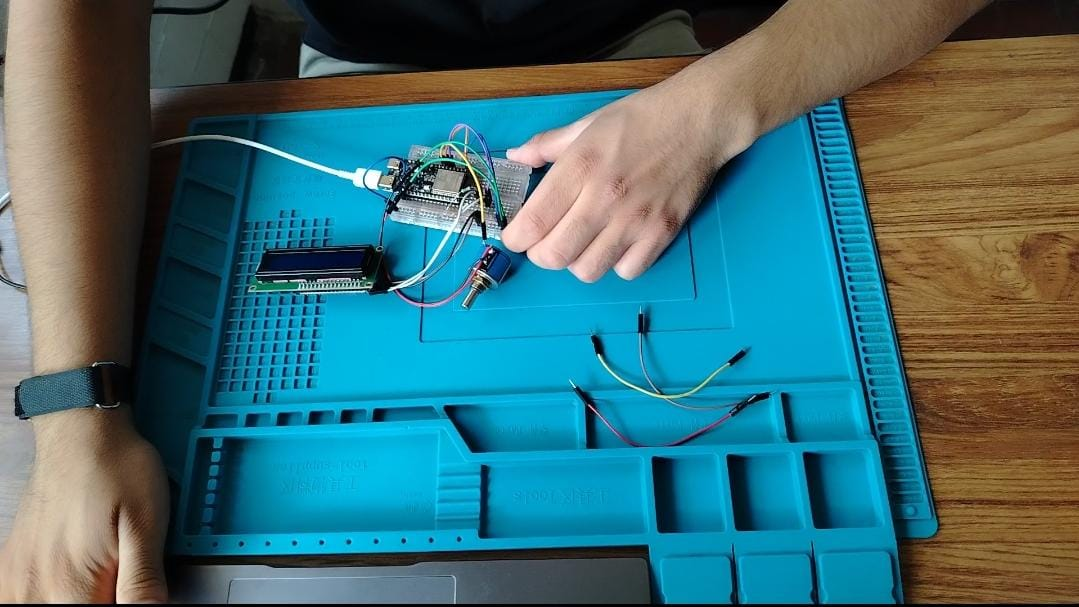
\includegraphics[trim = {0mm 0mm 0mm 0mm},clip,scale=0.2]{12/Img/evidencia3.jpg}
            \caption{Evidencia del proceso de ensamble}
            \label{fig:evidencia3}
    \end{figure}
    
    \begin{figure}[H]
            \centering
            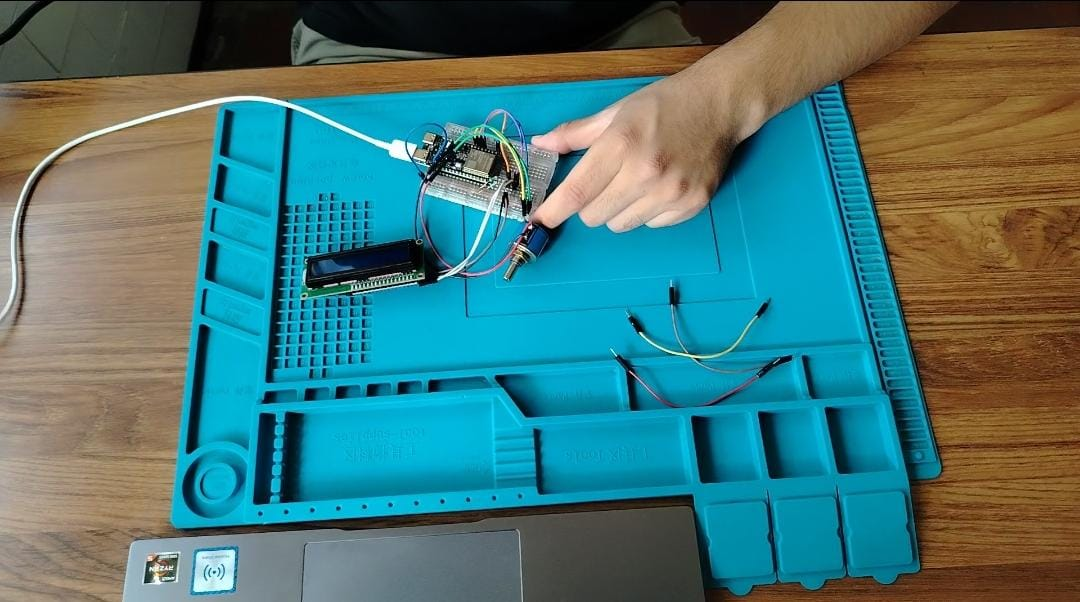
\includegraphics[trim = {0mm 0mm 0mm 0mm},clip,scale=0.2]{12/Img/evidencia4.jpg}
            \caption{Evidencia del proceso de ensamble}
            \label{fig:evidencia4}
    \end{figure}
    %Antes de comenzar a preparar tu artículo, es importante que lea primero la guía del autor, la cual incluye los temas o apartados que son necesarios para tener tu trabajo completo.
    %Una vez completada la edición del texto, el documento está listo para el uso de esta plantilla. En este archivo recién creado, resalte todo el contenido e importe el archivo de texto preparado. Ahora esta listo para estilizar su documento.
    %En esta sección se deben presentar todo lo obtenido de la sección 2, incluidas deducciones o efectos del desarrollo. También se podrán incluir subsecciones numeradas de la siguiente forma:
    
    \subsection{Autores y Afiliaciones}
    
    Para distinguir las afiliaciones de los autores, utilice superíndices iniciando con el número 1, 2, etc., sucesivamente, esto dependerá de la cantidad de los departamentos a los que estén afiliados los autores. En caso de que todos los autores pertenezcan a una mismo departamento e institución, utilizar sólo el superíndice 1. 
    
    \subsection{Identificar los encabezados}
    
    Se les recuerda a los autores que los encabezados deben de estar conforme los solicita la guía del autor. De ahí se puede adaptar el trabajo para que sea más fácil de entender para el lector.
    Los encabezados organizan los temas sobre una base relacional y jerárquica. Por ejemplo, el título del documento es encabezado del texto principal porque todo el material posterior se relaciona y elabora sobre este tema. 
    
    \subsection{Tablas y Figuras}
    
    \begin{enumerate}
        \item Posición de las tablas y figuras: Coloque las figuras y las tablas en la parte superior e inferior de las columnas. Evite colocarlos en medio. Las figuras y las tablas grandes pueden abarcar ambas columnas. Los títulos de las figuras deben de estar debajo de las mismas; los títulos de las tablas deben aparecer encima de ellas. Insértese las figuras y los cuadros después de citarse en el texto. Utilice la abreviatura “Fig. 1”, incluso al principio de una oración. 
    \end{enumerate}
    
    \section{Conclusiones}
    
    Se describe aquí el alcance del trabajo, logros obtenidos y perspectivas para el futuro de este. Se sugiere colocar información cuantitativa obtenida.
    
    \section{Agradecimientos}
    
    Es importante darles su debido reconocimiento a los laboratorios, instituciones, organizaciones, entre otros que han sido participes para la culminación de este trabajo. También es importante mencionar, fondos, proyectos, becas, entre otros que se le han otorgado al o los autores para realizar el trabajo de investigación. Ejemplo: “Los autores agradecen al Concejo Nacional de Ciencia y Tecnología por los recursos otorgados…”
    
    \section*{Referencias}
    \cite{REF2}
    \cite{REF4}
    \cite{REF5}
    \cite{REF6}
    \cite{REF7}
    \cite{REF8}
    \cite{REF9}
    %Para esta platilla, se solicita al autor enumerar las citas de manera consecutiva entre corchetes \cite{YLi2013}. 
    %La puntuación de la oración que sigues sería \cite{Mesaelides2011}. 
    %Refiérase simplemente al número de referencia, como en \cite{Morales2012}, no utilice “Ref. [3]” o “referencia [3]” excepto al principio de una oración: “La referencia [3] fue la primera…”
    %Enumere las notas al pie por separado en superíndices. Coloque la nota de pie de en la parte inferior de la columna en la que se citó. No coloque notas al pie en la lista de referencias. Utilice letras para las notas al pie de la tabla.
    %A menos de que haya tres autores o más; no utilice “et al.”. Los trabajos que no hayan sido publicados, incluso si han sido presentados para su publicación, deben ser citados como “inéditos”. Los trabajos que han sido aceptados para su publicación deben de citarse como “en prensa”. Poner en mayúscula sólo la primera palabra de un título, excepto los nombres propios y los símbolos de elemento. 
    %Otros ejemplos \cite{LAAngeles2021}, \cite{LAAngelesConni}. 
    %Véase el archivo adjunto \ref{anexo:pines}.
    
    % Ejemplo
    %  @Article{article,
    % 	author = "Author1 LastName1 and Author2 LastName2 and Author3 LastName3",
    % 	title = "Article Title",
    % 	volume = "30",
    % 	number = "30",
    % 	pages = "10127-10134",
    % 	year = "2013",
    % 	doi = "10.3389/fnins.2013.12345",
    % 	URL = "http://www.frontiersin.org/Journal/10.3389/fnins.2013.12345/abstract",
    % 	journal = "Frontiers in Neuroscience"
    % }
    
    % @book{book,
    %   author    = {Author Name}, 
    %   title     = {The title of the work},
    %   publisher = {The name of the publisher},
    %   address   = {The city},
    %   year      = 1993,
    % }
    
    % @incollection{chapter,
    %   author       = {Bauthor Surname}, 
    %   title        = {The title of the work},
    %   editor       = {Editor Name},
    %   booktitle    = {The title of the book},
    %   publisher    = {The name of the publisher},
    %   address      = {The city},
    %   year         = 2002,
    %   pages        = {201-213},
    % }
    
    % @InProceedings{conference,
    %   author = {Cauthor Name and Dauthor Surname and Fauthor LastName},
    %   title = {The title of the work},
    %   booktitle = {The title of the conference proceedings},
    %   year = 1996,
    %   publisher = {The name of the publisher},
    %   editor = {Editor Name1 and Editor Name2},
    %   pages = {41-50},
    % }
    
    % @book{cho,
    %   author       = {Gauthor Name1}, 
    %   title        = {The title of the work},
    %   publisher = {Country code and patent number},
    %   address      = {Patent Country},
    %   year = 2013
    % }
    
    % @book{patent,
    %   author    = {Hauthor Surname1}, 
    %   title     = {The title of the work},
    %   publisher = {Patent number},
    %   address   = {Patent country},
    %   year      = 2010,
    % }
    
    % % please use misc for datasets
    % @misc{dataset, 
    % 	author = "Author1 LastName1 and Author2 LastName2 and Author3 LastName3",
    % 	title = "Data Title",
    % 	year = "2011",
    % 	doi = "10.000/55555",
    % 	URL = "http://www.frontiersin.org/",
    % }
    
    \bibliographystyle{ieeetr}
    \bibliography{12/referencias}
    % 
    % 
    %%%%%%%%%%%%%%%%%%%%%%%%%%%%%%%%%%
    \appendix
    %%%%%%%%%%%%%%%%%%%%%%%%%%%%%%%%%%
    % 
    % 
    \centering{\section[\appendixautorefname{}]{Apéndice}}\label{anexo:listaMateriales}
    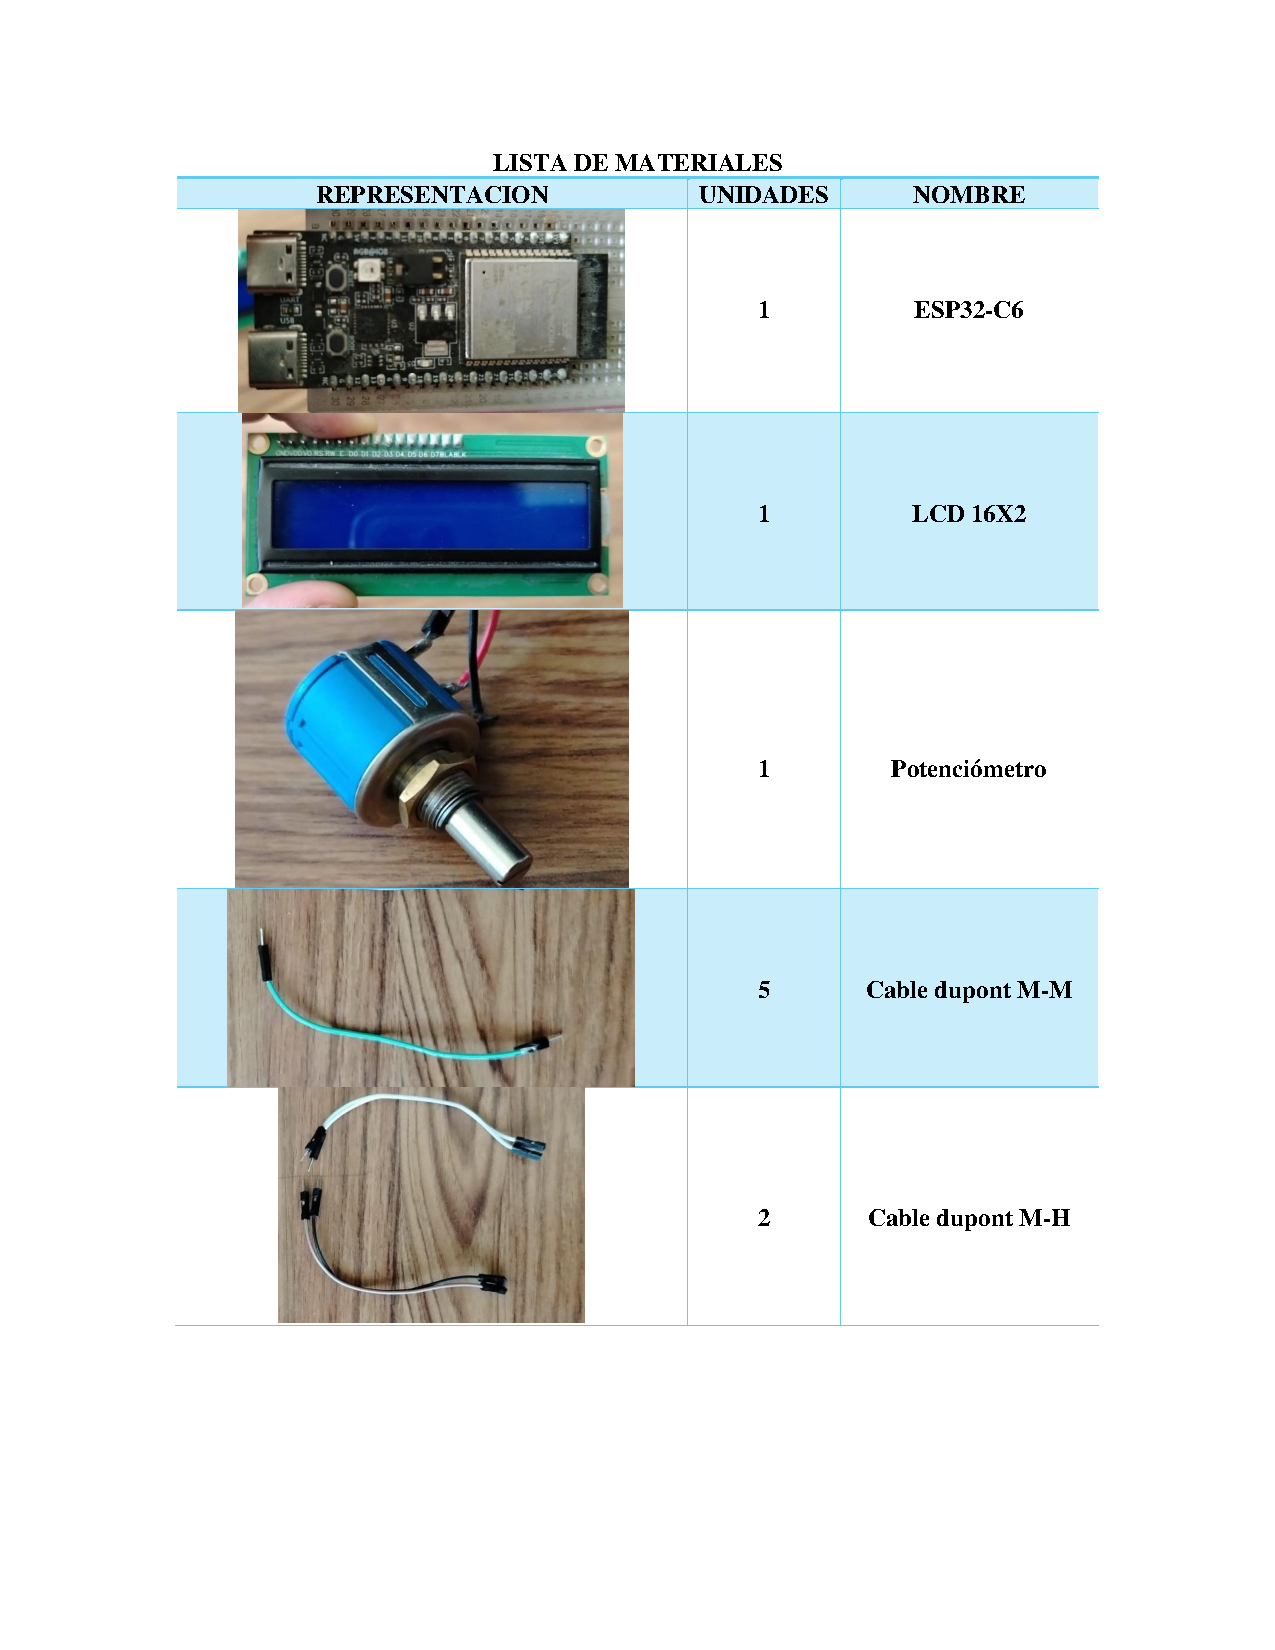
\includepdf[pages=-]{12/Img/listaMateriales.pdf}
    \centering{\section[\appendixautorefname{}]{Apéndice}}\label{anexo:guiaEnsamble}
    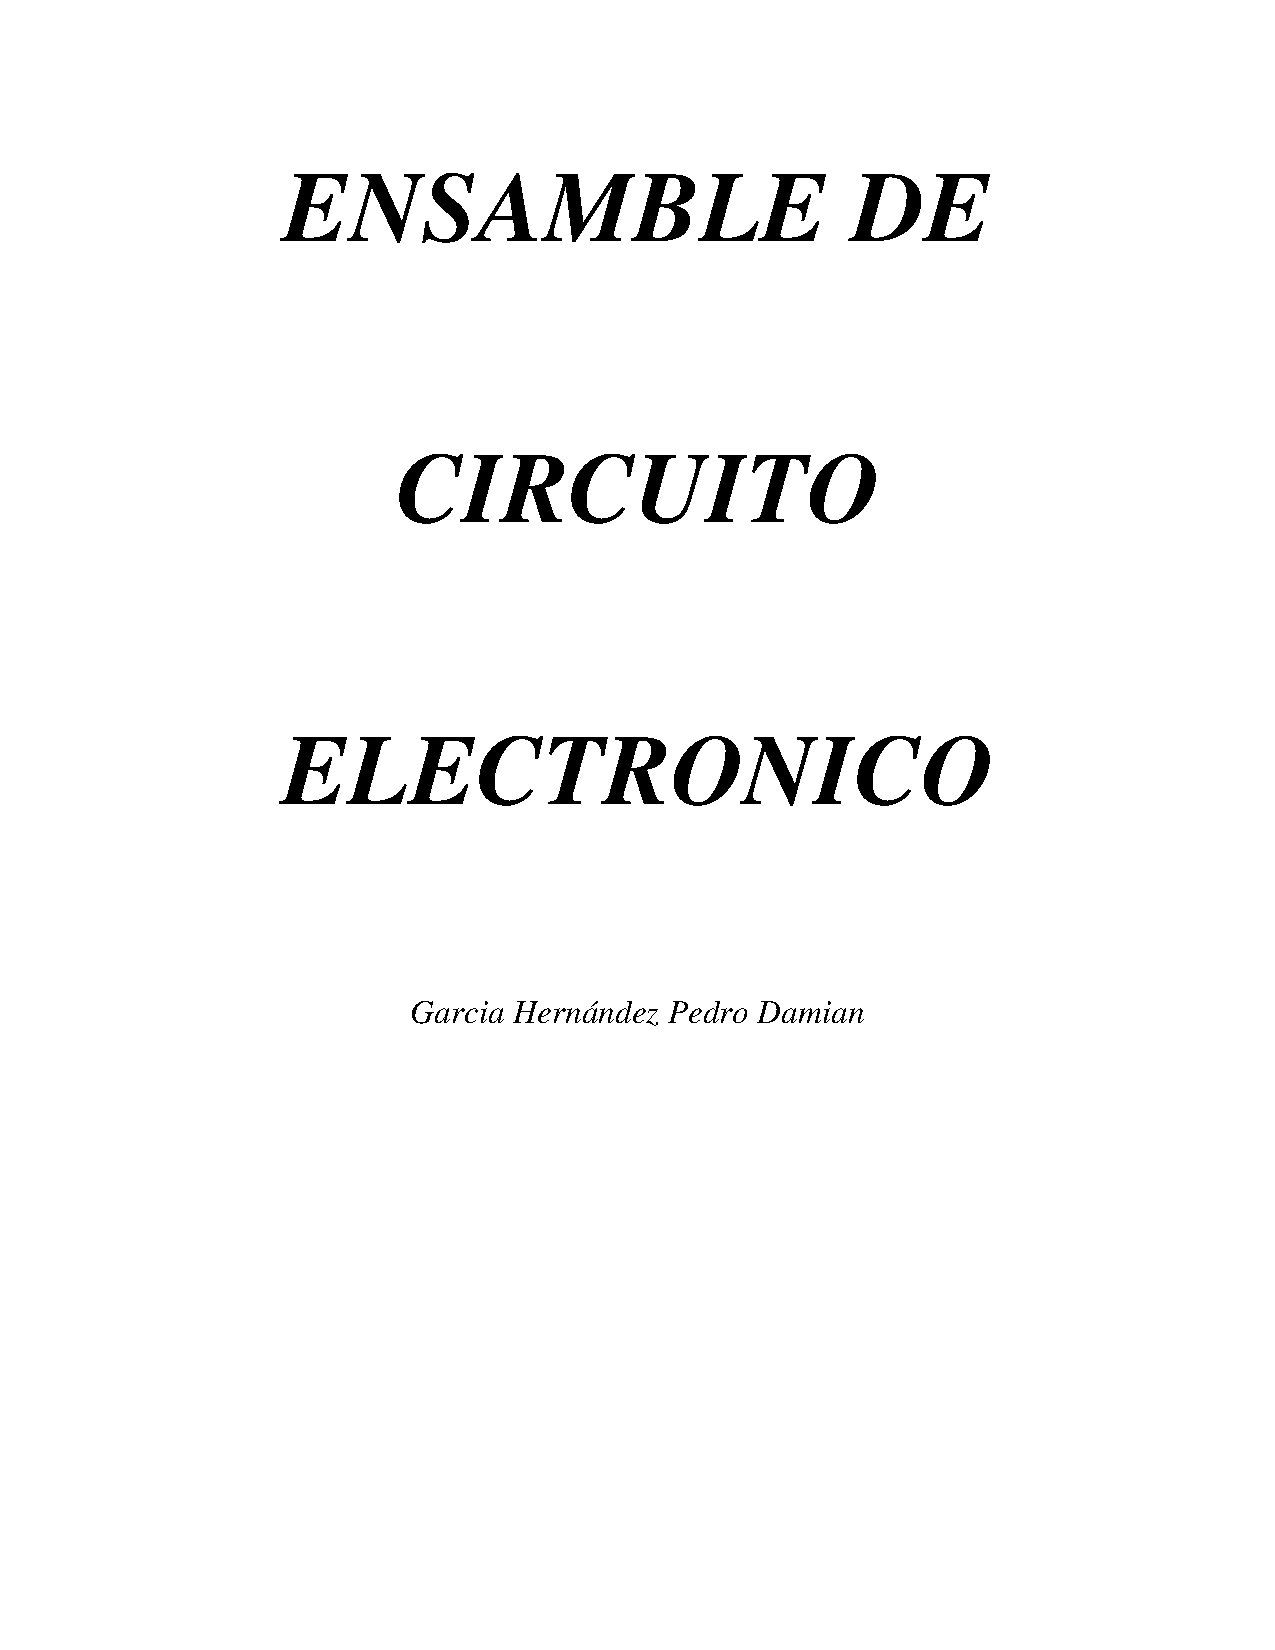
\includepdf[pages=-]{12/Img/guiaEnsamble.pdf}
    %%%%%%%%%%%%%%%%%%%%%%%%%%%%%%%%%%%%%%%%
    